\documentclass[draft]{tudelft-report}
% \documentclass{tudelft-report}
\usepackage{gensymb}
\usepackage{changes}
\usepackage{booktabs}
% \usepackage{lscape}
% \usepackage{pdflscape}
\usepackage[style=authoryear,maxcitenames=2,maxbibnames=100,giveninits=true]{biblatex}
\usepackage{csquotes}
\usepackage[author=Max,final]{pdfcomment}
\usepackage{siunitx}
\usepackage{pstricks}
\usepackage{import}
\usepackage[acronym]{glossaries}
\usepackage[section]{placeins}
% \usepackage{floatrow}
% \usepackage{tablefootnote}
\addbibresource[datatype=bibtex]{library.bib}
\addbibresource[datatype=bibtex]{non-mendeley.bib}

% copied from https://tex.stackexchange.com/questions/6850/table-and-figure-side-by-side-with-independent-captions
\newfloatcommand{capbtabbox}{table}[][\FBwidth]

\begin{document}

% \showthe\textwidth % pt.
%% Use Roman numerals for the page numbers of the title pages and table of
%% contents.
\frontmatter
% \pdfcomment{decide on consistent hyphenation of remote sensing, signal finding, etc}
% \pdfcomment{make sure that acronyms are defined the first time they're used}
% \pdfcomment{check for consistent spelling of Bayesian, kriging, etc}
% \pdfcomment{check for contractions}
%% Uncomment following 16 lines for a cover with a picture on the lower half only
\title{Bayesian downscaling of global bathymetry using spaceborne lidar}
% \subtitle[tudelft-black]{}
\author{M.\ A.\ E. Lindsay}
\affiliation{Technische Universiteit Delft}
\coverimage{figures/my_spacelidar_image/cover_image2.pdf}
% \covertext[tudelft-white]{
%     \textbf{Draft as of \today} 
%     % possibly \\
%     % spanning 
%     % multiple 
%     % lines
%     % \vfill
%     % ISBN 000-00-0000-000-0
% }
% \setpagecolor{tudelft-cyan}
\definecolor{title}{HTML}{4884d6}
\makecover


%% Include an optional title page.
\begin{titlepage}


    \begin{center}

        %% Insert the TU Delft logo at the bottom of the page.
        
        %% Print the title in cyan.
        {\makeatletter
            \largetitlestyle\fontsize{48}{94}\selectfont\@title
            % \largetitlestyle\color{tudelft-cyan}\Huge\@title
            \makeatother}
        
        %% Print the optional subtitle in black.
        {\makeatletter
            \ifx\@subtitle\undefined\else
                \bigskip
                {\tudsffamily\fontsize{22}{32}\selectfont\@subtitle}
                %\titlefont\titleshape\LARGE\@subtitle
            \fi
            \makeatother}
        
        \bigskip
        \bigskip
        
        by
        %door
        
        \bigskip
        \bigskip
        
        %% Print the name of the author.
        {\makeatletter
            %\largetitlefont\Large\bfseries\@author
            \largetitlestyle\fontsize{26}{26}\selectfont\@author
            \makeatother}
        
        \bigskip
        \bigskip
        
        to obtain the degree of Master of Science
        
        at the Delft University of Technology,
        
        \pdfcomment{add this}
        to be defended publicly on %Tuesday November 3, 2022 at 10:00 AM.
        
        \vfill
        \begin{tabular}{lll}
            Student number:   & 5243610                                                                          \\
            Project duration: & \multicolumn{2}{l}{March 1, 2022 -- ?}                          \\
            Thesis committee: & Prof.\ dr.\ ir.\ S.\ Aarninkhof,                        & TU Delft, Chair        \\
                              & Dr.\ ir.\ B.\ Wouters,     \pdfcomment{prof? double check}                                  & TU Delft, Supervisor   \\
                              & Dr.\ ir.\ A.\ Gijón-Mancheño,                                & TU Delft               \\
                              & Dr.\ ir.\ G.\ de Boer,                                       & Van Oord, Supervisor 
        \end{tabular}
        %% Only include the following lines if confidentiality is applicable.
        
        \bigskip
        \bigskip
        % \emph{This thesis is confidential and cannot be made public until December 31, 2013.}
        
        \bigskip
        \bigskip
        % An electronic version of this thesis is available at \url{http://repository.tudelft.nl/}.
        Draft as of \today
        %\\[1cm]
        
        %\centering{\includegraphics{cover/logo_black}}
        
        
    \end{center}
    
    \begin{tikzpicture}[remember picture, overlay]
        \node (tud) at (current page.south)[anchor=south]{
            \includegraphics{cover/logo_black}
        };
    \end{tikzpicture}
    
    \begin{tikzpicture}[remember picture, overlay]
        \node at (current page.south)[anchor=south,above=2cm]{
            
\includegraphics[width=0.4\textwidth]{figures/VanOord-2048x785.png}
            
        };
    \end{tikzpicture}
\end{titlepage}


Nearshore bathymetry needs 

Accurate nearshore bathymetry data is essential for navigational safety, shore protection, and coastal engineering research. Inaccurate bathymetry is one of the most severe limitations on the accuracy of numerical wave modeling. Because high resolution data is not available in most of the world, nearshore wave modeling studies often rely on global bathymetry datasets like GEBCO. The ~500m horizontal resolution is not sufficient for accurate wave modeling. One potential source of higher resolution nearshore data is other spaceborne remote sensing, such as lidar satellites. This study investigates how additional data sources can be combined with GEBCO to create a higher-resolution, higher accuracy product.

Satellite-Derived bathymetry

Lidar satellites, like ICESat-2, have been shown to be able to penetrate the first few meters of the nearshore zone. This can provide bathymetric data coverage along limited areas after some processing to isolate bathymetric signal. Bathymetry can also be estimated using the spectral response from optical remote sensing satellites. The topic under investigation is if these remote sensing sources, and any additional public data sources, can be combined to produce a statistically upscaled version of GEBCO that would provide higher resolution coverage in the nearshore zone. To combine them, a Kalman updating technique is proposed. The Kalman update technique allows a combination of the measurements at each discrete point, which is weighted based on the margin of error of each measurement.

Method of data assimilation 

To implement the Kalman upscaling, first global data from GEBCO is clipped to an area of interest, and then interpolated bilinearly to 50m resolution. Then, the ICESat-2 photon data for the area is processed to find a series of point measurements containing bathymetric data. To fill in the gaps between these point measurements, the bathymetric points are subsampled and interpolated to the same resolution as the GEBCO data using ordinary kriging, which results in a raster of uncertainty, and a raster of the interpolated depth value. To update the interpolated GEBCO raster, the Kalman gain is calculated for each raster cell in an elementwise manner, and using the Kalman state equation a new bathymetry grid is produced. If other data is available, the process can be applied recursively with other depth and uncertainty grids, with the output depth and uncertainty of the first iteration used the input to the second iteration, and so on. The process can allow the accuracy and resolution of the global dataset to be increased, without needing any additional a priori data.

Validation

To validate the method, the RMSE error is calculated between the resulting bathymetry grid and previously validated, high accuracy survey data. The validation will be applied at several global test sites to verify that the method generalizable to other regions.

Outlook

The results of this research could allow easier methods of characterizing nearshore bathymetry in remote areas, and could also be extended to include temporal variation – as more bathymetric data becomes available, it could be used measure the dynamic changes coastal systems. Data with this temporal dimension would provide valuable validation data for coastal dynamics models.

\chapter*{Summary}

Bathymetric data is valuable because it is essential for nearly every aspect of coastal management and monitoring but is difficult to obtain, especially in the nearshore zone. Traditional techniques like acoustic sounding provide reasonably high-accuracy data, but survey campaigns are expensive and the survey vessels cannot operate in the shallowest areas of the nearshore zone. Airborne lidar surveying provides high resolution, high accuracy data in the shallowest waters, but the associated survey campaigns are extremely expensive and are very sensitive to environmental conditions. Because of the limitations of conventional survey techniques in the nearshore zone, there is much interest in ways of estimating bathymetry using only spaceborne remote sensing data. Spaceborne remote sensing data is advantageous because of wide global coverage and because the data is often publicly available.
\vskip 0.1in

Traditionally, there are two main techniques for extracting bathymetric estimates from satellite data. One approach, called optical satellite derived bathymetry (SDB), estimates the bathymetry based on the relationship between the attenuation of different parts of the visible light spectrum in the water column. These techniques require in-situ data to calibrate, and require the site to have water that is clear down to the seabed. The second approach is to use satellite imagery to estimate the wave field in a region, and then back-calculate the bathymetry based on the evolution of the wave field in space. This is called the wave-kinematic approach. This approach provides less accurate and lower resolution bathymetry estimates than optical SDB, and the deepest depth that can be estimated is limited by the maximum wavelength at the time of the satellite data acquisition. The advantage of wave-kinematic approaches is that the deepest estimation depth is not limited by water clarity.
\vskip 0.1in

NASA's ICESat-2 satellite is a lidar satellite that provides high-accuracy point elevations along linear transects all over the world. It was originally intended to study the elevation of ice in the polar regions, but researchers have discovered that it can sometimes also capture the elevation of the seabed in coasts with very clear water. This has led to a number of papers that extract bathymetric point data from ICESat-2 and use it in combination with optical SDB methods to produce a bathymetric estimate without requiring any in-situ data.  
\vskip 0.1in

Most of the prior studies that extract bathymetric point estimates from ICESat-2 look at a limited number of satellite passes (3--10), and either use manual extraction of the seabed signal based on the researcher's judgement, or use other semi-automated techniques that estimate the seabed based on the density of photons in the vertical direction that are manually checked before use. The goals of this project are to find ways to automate the signal extraction from ICESat-2 data so that it can be implemented at a larger scale (up to hundreds of transects), to evaluate how these sparse point measurements can be interpolated into a continuous gridded product, and to evaluate if this interpolated data can be combined with existing global datasets to add additional value by increasing the resolution and decreasing the error. 
\vskip 0.1in

The methodology proposed is split into 3 major parts. First, the data processing and signal extraction from the satellite data: For a given area of interest, the ICESat-2 data is downloaded and processed to extract only photons that are located in the nearshore zone. It is then corrected for the effect of light refraction in the water column. Then, points that are likely to be sea surface signal are extracted based on the density of photons in the vertical direction, estimated by applying a Kernel Density Estimation (KDE) function along a moving window of 100 adjacent photons. The second part of the method is to interpolate the resulting points into a continuous bathymetric surface via universal kriging, a geostatistical approach that takes into account the elevation at each point and the distance between them to produce a gridded output of the estimated interpolated surface and the confidence in the interpolation. The third step is to combine the interpolated surface with a prior estimate, in this case the global bathymetry dataset GEBCO, via a Kalman filter. The Kalman filter is a bayesian approach that takes into account the new estimate and the uncertainty. Areas of the interpolated data with high certainty (i.e., nearer to ICESat-2 point measurements) will have a larger impact on the prior estimate, whereas areas with a lower certainty will have a correspondingly lower magnitude of impact on the prior depth estimate.
\vskip 0.1in

To test the feasibility of the kriging and Kalman updating approach, a synthetic experiment is created using a one of validation data sets. Random point samples from the validation data are taken, and these point samples are used as input to the kriging and kalman updating process. For the study site evaluated here, it is found that by kriging these input points and then combining them with GEBCO data, the error of the combined product is lower than either the error of GEBCO or the kriging surface. The Kriging + Kalman updating approach is also validated using a subset of the JarKus dataset, a series of point measurements of bathymetry surveyed annually along the entire Dutch coast. These data points were used as input to the kriging process, and the output of the kriging process was combined with the prior estimate of the bathymetry (i.e, GEBCO) using the Kalman filter step. The combination of Kriging and Bayesian combination with existing data improves the estimate than either dataset alone, showing that the Bayesian combination approach can add value compared to existing data.
\vskip 0.1in

The entire processing chain is then tested at 4 test sites. The proposed signal extraction technique produced bathymetric point estimates with an RMSE between 0.54 m and 9.53 m at the various sites. The sites with the largest magnitude errors are due to errors in the photon filtering approach, which could be corrected by improving the land mask data. If the subsurface filtering errors are removed, the highest RMSE at a site is 2.42 m. After extracting the bathymetry points and applying the kriging and kalman updating techniques to produce the final output, a gridded product at higher resolution, some sites show a reduction in RMSE of up to 34\% compared to GEBCO. However, a few sites also show an increase in RMSE. This is due primarily to uneven and anisotropic distributions of ICESat-2 point bathymetry estimates at some sites; kriging depends on estimating trends in data, and if the points are not well-distributed in the site it results in a lower quality of the universal kriging interpolation surface.
\vskip 0.1in
To implement this approach at a global scale, the computational efficiency of the processing chain must be maximized. One way to increase the efficiency is to apply the KDE signal extraction step only to ICESat-2 transects that are the most likely to contain good quality bathymetric signal. Therefore, several ways of pre-selecting the most likely transects to provide good bathymetry signal are investigated. Because high water clarity is required for the lidar signal reach and be returned by the sea bed, the estimated Secchi depth along the ICESat-2 transect was found and compared to the results. No clear relationship between the Secchi depth and the RMSE of the lidar data along a transect was found. Several other transect metadata variables were also checked for their relationship with the transect RMSE; the mean fraction of fully saturated photons, the density of photons along the transect, and the percent of ocean surface photons classified as 'high-confidence' in the default photon classification provided by NASA. However, none of the variables were found to provide a clear way to filter out high-error transects while retaining the low-error transects.
\vskip 0.1in

The proposed processing chain has the potential to increase the horizontal resolution of GEBCO data from 500 m to 50 m while also decreasing the vertical RMS error by up to 35\% without requiring any manually-surveyed data. This result was achieved using the exact same input parameters to the processing chain for every study site; it is likely that the parameter choice could be further optimized to produce better results. The computational bottlenecks in the approach are the KDE signal finding step and the Kriging step. Currently, the approach is practical to implement on consumer computers with a study site of up to 500~$\text{km}^2$, but finding ways to pre-select the best transects could allow for significant efficiency gains in the KDE signal finding process. The approach is also limited by the need for exceptionally clear water to extract lidar bathymetric signal. Due to these characteristics, the processing chain proposed here could provide the basis for a global coral reef bathymetry data set.

\chapter*{Preface}
\setheader{Preface}

Preface\ldots

\begin{flushright}
{\makeatletter\itshape
    \@author \\
    Delft, January 2013
\makeatother}
\end{flushright}


\listofpdfcomments[liststyle=Comment]
\pdfcomment{check for captions that are too long, give them a different caption}
\listoffigures
\listoftables
\tableofcontents

%% Use Arabic numerals for the page numbers of the chapters.
\mainmatter
\parskip 0.1in
% smallchange
\chapter{Introduction}
\label{chapter:introduction}

An introduction.

% Reason

% Aim

% Structure

\chapter{Background}

% \pdfcomment{add secchi depth/ocean color section}

\section{Remote sensing of bathymetry}
There are several established methods for calculating bathymetric data from passive optical and SAR satellite data, and recent advances in cloud computing capabilities like Google Earth Engine (GEE) \parencite{Gorelick2017a} make large catalogs of remote sensing data more accessible \parencite{Pike2019,Turner2021}. The approaches can be broadly classified into \emph{wave-kinematic} and \emph{optical inversion} techniques.

\subsection{Wave-Kinematic bathymetry}
This approach uses the hydrodynamic properties of ocean surface to produce an estimate of the bathymetry in a 2D grid. Hydrodynamic variables such as wave celerity and wavenumber can be estimated from either optical or SAR satellite data. The bathymetry can then be calculated using the wave dispersion relation $c^2 = \frac{g}{k}\tanh{kh}$, which relates the wave celerity $c$ to the wavenumber $k$ and the depth $h$ \parencite{Almar2021e}. The major advantage of this method is that it does not require light to penetrate the water column. Therefore, it is not limited by water column properties such as turbidity, which can be a significant limitation to optical SDB methods along many coastlines. The disadvantages of this approach are that the horizontal resolution is limited compared to optical methods, and that the maximum depths where this approach can be applied is limited by the wavelength: longer waves feel the bottom earlier, so bathymetry estimates in deeper areas are only possible on coasts exposed to swell waves, which have a longer wavelength \parencite{Almar2021e}.

\subsection{Bathymetry from optical remote sensing}
Optical remote sensing is a passive technique, as it detects light from the sun reflected by the earth. Since the 1970s many methods of estimating bathymetry based on the optical quality of the water have been found, all based on the physical principle that water attenuates light. Optical methods require that the water is \emph{optically shallow}, or clear enough that light can reach the sea floor. This is a significant restriction, but in places where it is applicable it can provide continuous estimates of bathymetry with a resolution up to the resolution of the optical imagery. This means bathymetry grids at 10~m horizontal resolution using publicly available Sentinel-2 imagery, up to 0.5~m if commercial imagery is purchased \parencite{Babbel2021a,LeQuilleuc2022b,Pike2019}. There are two broad types of algorithms for extracting bathymetric data from optical satellite imagery, analytical and empirical. Empirical models link the amount of attenuation of each pixel to in-situ depth measurements and derive a relationship between color and depth. One advantage is that empirical approaches are generally computationally inexpensive. Analytical or physics-based approaches require corrections for atmospheric and subsurface factors \parencite{Turner2021} and require more sophisticated computational capabilities to apply.

Empirical optical methods require some in-situ data to establish the relationship between the optical properties and the depth in the area. \cite{Parrish2019} conclude that the most effective way to use ICESat-2 data for bathymetric estimation is to combine it with optical techniques. Because the ICEsat-2 data provides relatively high accuracy point estimates, and optical methods allow the estimation of a 2D bathymetry grid but require in-situ point measurements for calibration, combining the two techniques provides a synergistic fusion of the strengths of both. There have since been several studies that employ this approach, and evaluate different techniques for correcting refraction, identifying bathymetry signal, and combining the lidar data with optical techniques (For examples of studies combining ICESat-2 with optical SDB methods, see \cite{Geyman2019,Pike2019,Ma2020,Lee2021,Albright2021,Ranndal2021,Gleason2021,Thomas2021d,Babbel2021a,Hsu2021,Cao2021,Xie2021,Surisetty2022,Zhong2022a,Zheng2022,Daly2022,Xu2022,Magruder2020,Thomas2022,LeQuilleuc2022b}). Suffice it to say this topic has seen significant interest from researchers in recent years.

\section{Lidar Bathymetric Surveying}

The earliest attempts to use Light Detecting and Ranging (lidar) to survey the coastal zone date back to the late 1960s. \parencite{Bailly2016}. The technology has matured significantly since then and currently airborne lidar using a strong 532nm laser beam is a common technique for high accuracy bathymetric and topographic surveying. The downside of this technique is that it does not scale well to large areas because it requires expensive equipment, and extensive post-processing work is needed after the survey to produce a final product. 

Recent advances in lidar technology have allowed the development of the photon-counting lidar, which requires significantly less energy to detect a return signal. These have allowed the practical application of constant lidar data collection in satellites. The use of spaceborne lidar is a more recent area of research, but some early results have shown that spaceborne lidar can find depths as deep as 38 m \parencite{Parrish2019}.

The potential for bathymetric mapping using spaceborne laser observations has been noted since before the advent of the ICESat-2 mission. The predecessor mission carried a lidar instrument called the Geoscience Laser Altimeter System (GLAS). GLAS was a green-light laser intended for measuring atmospheric aerosols \parencite{Abshire2005}. However, because of the laser architecture, GLAS was not able to penetrate the water column \parencite{Forfinski-Sarkozi2016}. However, a prototype of ATLAS, called the Multiple Altimeter Beam Experimental lidar (MABEL) instrument was tested with high-altitude aircraft missions, allowing a simulation of the data that would be provided by ATLAS \parencite{Mcgill2013}. Early experiments with MABEL showed good agreement between bathymetric measurements from MABEL and high-quality airborne reference data \parencite{Jasinski2016,Forfinski-Sarkozi2016}.

To detect the relatively weak signal reflected off the seafloor, very clear water and ideal atmospheric and oceanic conditions are required. Therefore, only a fraction of transects contain bathymetric signal even for ideal sites. One of the most important considerations to use underwater lidar data is the method of finding bathymetric signal while rejecting noise. One known property of the bathymetric signal is that a relatively high density of returns in the vertical (Z) direction. 

\section{Geodetic reference systems for oceanography}

The ICESat-2 photon heights are by default referenced to the WGS84 ellipsoid. To convert these to an approximate mean sea level, some geodetic correction is required. The \emph{geoid} is defined as a level surface that is normal to the gravitational acceleration at every point. It is not just the surface of equal gravitational potential, but it also includes the centrifugal force due to a fixed local reference frame. The geoid can be defined as a level surface in a theoretical potential field $W$ such that $g= - \nabla W$. More intuitively, it can also be defined as the surface where the ocean surface would settle if it was in static equilibrium. \parencite{Hughes2008}.

The contours of the geoid can be estimated using satellite gravimetry, and from these measurements the shape of the geoid can be mathematically approximated by a sum of a series of spherical harmonic functions.

The surface of the actual geoid changes with over time due to deformation of the earth induced by the gravitational forcing from the Sun and the Moon. Because the gravitational forcing of both the sun and the moon has both periodic and non-periodic components, the time average of their effect is non-zero. This time-averaged deformation is called the \emph{permanent tide}. For satellite altimetry, a reference system that changes with time can be inconvenient, so measured heights are often reported in a coordinate system that is referenced to the \emph{tide-free geoid}. The tide-free geoid is a theoretical reference surface that removes both the periodic effect and the permanent tide \parencite{Makinen2009}. It can be thought of as the gravitational potential of the Earth if the distance to the sun and moon was increased to infinity.

\subsection{Inverted barometer effect and dynamic atmosphere correction}

The instantaneous sea surface elevation is affected by the local weather and atmospheric conditions. The Inverted barometer (IB) effect refers to the effect of air pressure on the ocean height, or the  local dynamic sea-surface topography \parencite{Robbins2022}. Spatial gradients in air pressure due to local high and low pressure systems are equalized by gradients in the water surface height. When atmospheric pressure is low, the ocean level rises, and when atmospheric pressure increases it pushes the ocean surface down.

In the simplest formulation, the drop in ocean level is approximately 1cm per additional mbar of atmospheric pressure: $D_h \approx 0.99484(P_i-P_{ref})$, where $P_i$ is the instantaneous pressure in mbar and $P_{ref}$ is an assumed average pressure (1013.3 mbar) \parencite{Neumann2019e}

In addition to surface height changes due to atmospheric pressure forcing, the local wind stress field also creates gradients in the sea surface height due to water mass momentum forcing. These variations are higher frequency compared to the pressure forcing that is captured by the IB correction.

The combined effect of the IB effect and local wind forcing can be modeled using a global wave model that is forced using weather data. The combined correction factor is called the Dynamic Atmospheric Correction (DAC). The DAC correction provided in the ATL03 data product is sourced from the MOG2D model \parencite{LeProvost1994}, provided by AVISO. It is a global, barotropic, non-linear model of the world's oceans. It has a variable grid resolution to provide higher resolution data in coastal areas and enclosed seas. The MOG2D model is forced using the wind velocity and atmospheric pressure at 10 m height from the European Centre for Medium-Range Weather Forecasts (ECMWF) global weather model. The MOG2D model provides the DAC correction factor with a 6 hour temporal resolution and a $0.25^{\circ}$ horizontal resolution. These DAC values are interpolated in space and time to the nearest reference photon for inclusion in the ATL03 data product. The magnitude of the DAC correction factor is $\pm 50 cm$ in the vertical direction.


\section{ICESat-2}

The ICESat-2 mission is intended to gather high resolution topographic data on a global scale. The satellite carries the Advanced Topographic Laser Altimeter System (ATLAS). ATLAS is a highly sensitive photon-counting, green-light lidar. The satellite instrument points at Reference Ground Tracks (RGT) along the earth's surface, and returns with a repeat time of 91 days. Along the reference track, there are 3 beams, one pointing directly at the reference track, and two that are offset by approximately 3km on either side. Each of these three beams is further split into a weak and strong. The layout of the beams relative to the RGT are shown in Figure \ref{fig:icesat-rgts}, and the orientation of the spacecraft in 3D is shown in Figure \ref{fig:3d-beams}

\begin{figure}[htbp]
      \begin{floatrow}
            \ffigbox{\includegraphics[width=0.5\textwidth]{./figures/ATLAS_beam_layout_from_user_guide.png}}{\caption{Layout of the ICESat-2 beams relative to the Reference Ground Track}\label{fig:icesat-rgts}}
            \ffigbox{\includegraphics[width=0.5\textwidth]{./figures/3d_beam_view_from_atl03ATBD.png}}{\caption[The layout of the ICESat-2 beams in 3D space]{The layout of the ICESat-2 beams in 3D space. From \cite{Neumann2019d}}\label{fig:3d-beams}}
      \end{floatrow}
\end{figure}

Each of the 3 beams is split into a strong and weak beam, with the strong beam being approximately 4x more powerful \parencite{Neumann2019d}. With each laser pulse the instrument emits \(10^{14}\) photons which travel to the earth where they are reflected. For more reflective surfaces like snow and ice, up to 10 make it back to the sensor and are detected. For less reflective surfaces such as the open ocean, only 0-4 photons are detected at the satellite \parencite{Neumann2019d}. The exact number of emitted photons that return to the sensor and are detected at the sensor depends on the local atmospheric conditions and the reflectivity of the surface \parencite{Neumann2019e}. The highly sensitive instrument also receives significant noise, due to atmospheric scattering and photons from the sun. In clear water, some photons can travel to the bottom of the water and return. In water with a high suspended sediment concentration, these photons are more likely to be reflected higher in the water column \parencite{Ranndal2021}.
% \pdfcomment{per mom: water column graphic?}

The main mission of the satellite is to gather data about mass and elevation changes in ice sheets and glaciers, and to study global canopy height \parencite{Markus2017}. As part of the vegetation height mission, the observatory is sometimes pointed away from the reference ground track when flying over land. This increases the spatial density of the observations of vegetation height \parencite{Markus2017}. This operation, called \emph{offpointing}, begins before the satellite begins to record data over land, so the nearshore coastal area is also included, and therefore bathymetric and hydrological applications also benefit from increased spatial coverage \parencite{Magruder2021}.

To locate the position of each photon in 3D space, the time of flight of the photon is calculated with a precision of 800 ps \parencite{Neumann2019d}. The location of the center of mass of the instrument is found using Global Positioning System (GPS) systems onboard the satellite. By combining the measured time of flight and satellite position and attitude, the geolocation of each returning photon is calculated \parencite{Neumann2019d}.


\begin{figure}[!ht]
      \centering
      \includegraphics[width=0.5\textwidth]{figures/Meantide_vs_tide_free_comparison_doc.png}
      \caption{Relative levels of the reference planes}
      \label{fig:geoids-ellipsoids-graphics}
\end{figure}

Figure \ref{fig:geoids-ellipsoids-graphics} shows the various reference systems used in calculating the height of an individual photon in the ICESat-2 data production. The location of the satellite is resolved in ellipsoidal coordinates using the Precision Orbit Determination (POD) module. Then, using the travel time between the photon and the satellite, the location of the photon is calculated using the speed of light and corrections for atmospheric delays, instrument bias, and wave height. The ellipsoidal height of a photon located directly below the instrument nadir is calculated by the difference:

% \pdfcomment{this is range, actual location is needs to be adjusted further}

\begin{equation}\label{eq:raw_photon_calculation}
      H_{satellite_{surface}} = c(t_T-t_R)/2
\end{equation}
\begin{equation}
      H_p = H_{satellite_{ellipsoid}} - H_{satellite_{surface}}
\end{equation}
Where:
\begin{itemize}
      \item $H_{photon}$ is the height of the photon above the ellipsoid
      \item $H_{satellite_{ellipsoid}}$ is the height of the satellite above the ellipsoid (the brown line in figure \ref{fig:geoids-ellipsoids-graphics})
      \item $H_{satellite_{surface}}$ is the height of the satellite above the surface (the green line in \ref{fig:geoids-ellipsoids-graphics})
      \item $c$ is the speed of light
      \item $t_T$ and $t_R$ are the photon transmit and receive times respectively
\end{itemize}

This gives the height of a photon directly at the nadir of the satellite; since photon are actually collected along 6 different beams at various angles, the actual X,Y,Z location of the photon is triangulated based on the angle of the beam. 

The ATL03 data product reports the photon heights relative to the WGS84 reference ellipsoid. These ellipsoidal heights already include corrections for the solid earth tides, ocean loading, ocean pole tides, and atmospheric delays.

The height provided in the ATL03 data product is calculated by equation:

\begin{equation}
      H_{GC} =  H_{P} - H_{OPT} - H_{OL} - H_{SEPT} - H_{SET} - H_{TCA}
\end{equation}
Where:

\begin{itemize}
      \item \(H_{GC}\) is the geophysically corrected photon height above the WGS84 ellipsoid
      \item \(H_{P}\) is the uncorrected photon height above the WGS84 ellipsoid, from equation \ref{eq:raw_photon_calculation}
      \item \(H_{OPT}\) is the height of the ocean pole tide correction, which is the deformation at the poles induces by centrifugal effects of variations in the earth's rotational axis.
      \item \(H_{OL}\) is the height of the ocean loading tide, which is the deformation of earth's crust due to the weight of ocean tides
      \item \(H_{SEPT}\) is the height of the solid earth pole tide
      \item \(H_{SET}\) is the solid earth tide, the deformation of the earth's crust due to the gravitational effects of the sun and the moon
      \item \(H_{TCA}\) is the height of the total column atmospheric delay, which is the effect of atmospheric conditions the photon travel time.
\end{itemize}

$H_{GC}$ is the height above the WGS84 ellipsoid. To convert this ellipsoidal height into a value that can be used for computing the bathymetry, it needs to be converted into an instantaneous sea surface height. The equation that relates these is:

\begin{equation}
      H_{inst} = H_{GC} - H_{geoid} - H_{free2mean} - H_{DAC} - H_{tide}
\end{equation}

Where:
\begin{itemize}
      \item $H_{geoid}$ is the height of the tide-free geoid above the reference ellipsoid
      \item $H_{free2mean}$ is the difference between the tide-free and the mean-tide geoid
      \item $H_{DAC}$ is the dynamic atmospheric correction factor which includes periodic effects like local wind forcing
\end{itemize}

% The height value reported in ATL03 does not include the geoid or any tides. To find these values from the reported ellipsoidal height, the dataset includes correction factors for the tide-free geoid, the height difference between the tide-free and mean-tide geoid, and the height of the tide relative to the mean tide geoid as calculated by the GOT4.8 model. The mean sea level can be estimated by adding these correction factors to the ellipsoidal height. However, the GOT4.8 model tidal height is a based on a relatively low resolution grid, and therefore is less accurate in nearshore coastal areas and within embayments \parencite{Neumann2019e}.

\subsection{ICESat-2 data processing levels}

ICESat-2 data is provided to the public at a number of different processing levels. NASA provides a number of processing chains that produce higher-level products for different uses. The raw data transmitted from the satellite is considered to be Level 0. The NASA NSIDC decompresses this level 0 data, orders it in time and formats it in the HDF5 file format, and it is made available as a level 1 product, the lowest-level data that is available to the public.

In the level 2 products, the photon flight times are corrected for atmospheric effects, and the actual photon locations are resolved, then geodetically transformed to coordinates in WGS-84 ellipsoidal units.

In accordance with the scientific mission of the satellite, the level 2 product is then transformed into a number of higher-level products, each for a specific use case. Level 3 is divided into two sublevels, 3A and 3B. 3A products are point elevations of Land Ice, Sea Ice, Land vegetation, inland water elevation and ocean surface elevation. These point measurement products are then further transformed into level 3B or gridded products, which aggregate the point measurements over time to a grid.


\subsection{Weak vs. strong beams}

The beams are divided into weak and strong signals to enhance the radiometric dynamic range. The strong beams are expected to provide better signal-noise ratios over low-reflectivity surfaces, like the ocean and seafloor, while the weak beams are better for capturing very high reflectivity surfaces like ice, which might otherwise saturate the sensor and do not provide usable measurements \parencite{Neumann2019d}. The strong beams have been found to provide the better data for lidar bathymetry measurements, but the weak beams can still contain useful bathymetry data \parencite{Hsu2021}.


\subsection{Refraction correction}

The locations calculated by the data products from the satellite do not correct for the refraction induced by the water column. The subsurface photons are geolocated as if they are not underwater. However, because the speed at which light travels is different in water than the atmosphere. This effect introduces both a horizontal and vertical error in the photon location, as shown in Figure \ref{refract-image}.

When the instrument is pointed directly at the reference ground track, the laser beams point nearly directly at the satellite's nadir. When directly on-nadir, the additional horizontal error induced by refraction is $\sim 9~cm$ \parencite{Parrish2019}, which for bathymetric purposes is negligible. Some studies of bathymetry extraction from ICESat-2 data only use data that is collected when the instrument is pointing on-nadir, and therefore only correct for the vertical error using Snell's law.

However, by design ATLAS is capable of pointing up to $5 \degree$ off-nadir, or $\sim43~km$ away from the RGT \parencite{Magruder2021}. During offpointing, the horizontal error is more significant and must be corrected for accurate bathymetry \parencite{Parrish2019}. \citeauthor{Parrish2019} propose a method to correct for both horizontal and vertical error that is widely cited in later papers. The Parrish method assumes a flat water surface, but other studies have extended their method to include the effect of water slope or wave action on the refraction error \parencite{Ma2020,Zhang2022}.  This is referred to as \emph{first order} refraction correction in the table summarizing previous research (Table \ref{tab:researchsummary}).


\begin{figure}[!ht]
      \centering
      \includegraphics[width = 0.5\textwidth]{figures/refraction_error.png}
      \caption{The geometry of the error induced by refraction at the air-water interface. From \cite{Parrish2019}}
      \label{refract-image}
\end{figure}

The method proposed by \citeauthor{Parrish2019} is outlined below. Figure \ref{refract-image} shows some of the geometric variables used in the equations. First, the angle of refraction $\theta_2$ is calculated based on the relative speed of light in the air and water. This first step, shown in equation \ref{eq:snellslaw}, is the application of Snell's law.

\begin{equation}\label{eq:snellslaw}
      \theta_2 = \sin^{-1}{\frac{n_1 \sin{\theta_1}}{n_2}}
\end{equation}

The relative length of R and S are described by the ratio:
\begin{equation}
      R = \frac{S n_1}{n_2}
\end{equation}
Then the horizontal and vertical distance length corrections $\Delta Y$ and $\Delta Z$ can be calculated by the law of sines:
\begin{equation}
      S = \frac{D}{\cos{\theta_1}}
\end{equation}

\begin{equation}
      \gamma = \frac{\pi}{2} - \theta_1
\end{equation}

\begin{equation}
      \alpha = \sin^{-1}{\frac{R \sin{\phi}}{P}}
\end{equation}

\begin{equation}
      P = \sqrt{R^2 + S^2 - 2RS \cos{(\theta_1 - \theta_2)}}
\end{equation}

\begin{equation}
      \beta = \gamma - \alpha
\end{equation}

The horizontal correction $\Delta Y$ is along the direction of the laser pointing vector projected on to the earth's surface. To get the distance in local, rectangular coordinates that can used to correct the easting and northing coordinates in a local UTM system, $\Delta Y$ is projected onto the local coordinate system using the azimuth of the laser pointing vector $\kappa$.
\begin{align}
      \Delta Y & = P \cos{\beta}         \\
      \Delta Z & = P \sin{\beta}         \\
      \Delta E & = \Delta Y \sin{\kappa} \\
      \Delta N & = \Delta Y \cos{\kappa}
\end{align}


The curvature of the earth can also affect the accuracy of the refraction correction. For longer transects, this effect can be corrected with an additional correction suggested by \citeauthor{Parrish2019}. The equation for this correction factor is

\begin{equation}
      \delta \theta_{EC} = \arctan{\frac{H \tan{\theta_1}}{R_e}}
\end{equation}


\subsection{Extraction of bathymetric signal from photon data}\label{subsec:signal-finding}
The ATL03 data product includes a calculated confidence that a given photon return is signal or noise. The probability is assigned for each of the 5 surface types. Because bathymetric survey was not part of the original mission scope, there is no pre-calculated classification for subsurface returns. Therefore within the default classification bathymetric photons are often classified as noise. However, the classification of ocean surface classification is mostly reliable and can be used to filter out points near or above the sea surface \parencite{Ranndal2021}.

To find bathymetric signal, a separate algorithm specifically calibrated to distinguish bathymetric signal from noise photons is required. There are several different techniques proposed in the literature. Some early research on small sites used manual classification \parencite{Forfinski-Sarkozi2016,Thomas2021d,Babbel2021a,Albright2021}.

Other researchers have used implementations of the density-based spatial clustering for applications with Noise (DBSCAN) algorithm \parencite{Ester1996}, with parameters that are set adaptively based on the local density of returns, called \emph{adaptive DBSCAN} in the literature \parencite{Ma2020,Xie2021,LeQuilleuc2022b,Liu2021}.  \citeauthor{Thomas2022} created an algorithm called C-SHELPh, which uses a binned histogram approach to predict the location of the sea surface. \cite{Datta2021} proposed a method based on a kernel density estimation function. All of these automated classification approaches rely on the fact that when there is bathymetric signal present, the density of returns in the vertical direction is higher than in the surrounding area \parencite{Neuenschwander2019}.


\subsection{Summary of Prior Research on ICESat-2 derived bathymetry} %move to ICESat-2 section

Previous studies that have used bathymetry data extracted from ICESat-2 data are summarized in table \ref{tab:researchsummary}.

\begin{table}[h]
      \caption{Summary of prior studies that extract bathymetric data from ICESat-2 photons}
      \label{tab:researchsummary}
      % \centering
      \raggedright
      \begin{tabular}{rccccc}
            \midrule
            Paper                        & Year & Refraction Correction Method  & S/N Classification method \\
            \hline                                                                                          \\
            \citeauthor{Parrish2019}     & 2019 & Parrish method                & Manual                    \\
            \citeauthor{Ma2020}          & 2020 & Parrish + sloping sea surface & Adaptive DBSCAN           \\
            \citeauthor{Thomas2021d}     & 2020 & Parrish Method                & Manual                    \\
            \citeauthor{Albright2021}    & 2021 & First-order                   & Manual                    \\
            \citeauthor{Babbel2021a}     & 2021 & Parrish                       & Manual                    \\
            \citeauthor{Xie2021}         & 2021 & Parrish Method                & Adaptive DBSCAN           \\
            \citeauthor{Cao2021}         & 2021 & First-order depth correction  & A-DRAGANN                 \\
            \citeauthor{Lee2021}         & 2021 & Not specified                 & Not specified             \\
            \citeauthor{Liu2021}         & 2021 & Liu method                    & Adaptive DBSCAN    \\
            \citeauthor{Coveney2021a}    & 2021 & First-order                   & Manual                    \\
            \citeauthor{Datta2021}       & 2021 & Parrish                       & Watta                     \\
            \citeauthor{LeQuilleuc2022b} & 2022 & Parrish                       & DBSCAN                    \\
            \citeauthor{Thomas2022}      & 2022 & Parrish                       & C-SHELPh                  \\
            \bottomrule
      \end{tabular}
\end{table}



\chapter{Data Sources and Methods}\label{sec:methodology}
This chapter lays out the data sources and approach used for the project
\pdfcomment{Explain how my processing chain differs from the NASA one}
\pdfcomment{mention the UTM grid reprojection steps if they're not mentioned.}
\section{Data Sources}

The following section details the data sources were used as input to the processing chain.

\subsection{NASA ATL03 global geolocated photon data}

The main source of data is NASA's ATL03 V005 data product \parencite{icesat2data}. ATL03 is a level 1 data product that consists of the precise latitude, longitude, and elevation for each received photon. As a level 1 data product, it has already undergone some processing by the Atlas Science Algorithm Software (ASAS) to correct for instrument errors, to classify photons as likely signal or noise for different surface types, and to correct for some geophysical effects including earth tides to provide measurements relative to the WGS-84 ellipsoid. 

Additionally, the data includes variables that allow for further corrections and adjustments to change the height reference from the ellipsoidal height. These additional variables include correction factors for the tide, ocean surface depression due to atmospheric pressure, and factors to convert the ellipsoidal elevation to a height relative to the tide-free geoid.

The data is available via the National Snow and Ice Data Center Distributed Active Archive Center (NSIDC DAAC) via an Application Programming interface (API). The data is available divided into \emph{granules} that include several seconds worth of observations. The API allows searching for data based on spatial location and date of acquisition. Once the search has been completed, the resulting granules of ATL03 data can be downloaded. Before downloading, the data be further subset by spatial location, so that only photons within a geographic area are included. The granules can also be subset by variables, so that only specific variables of interest are included in the resulting download. This can significantly reduce the required download side if only a few variables are needed.


\subsection{GEBCO Global Grid 2021}

The General Bathymetric Chart of the Ocean (GEBCO) is a global grid of topography and bathymetry at a 30 arc-second mesh resolution \parencite{gebco2021griddata}. GEBCO is assembled by compiling many different data sources, including multibeam sonar data, nautical charts, and satellite gravimetric measurements for deep-ocean bathymetry \parencite{gebcocookbook}. The elevation data is referenced to a vaguely-defined 'mean sea level'. The various data sets included in GEBCO are all assumed to be referenced to MSL, but some datasets referenced to chart datum are included. 

GEBCO has a limited accuracy and resolution, but it is the only available data source in many places in the world, so it is sometimes used as the best-estimate in very data-poor sites. However, the accuracy of GEBCO varies depending on the input data sources. In this project, the GEBCO elevation is used both to filter locations that \emph{may} contain valid bathymetry, and used as a prior guess to the Bayesian updating approach. 

The elevation grid, and a metadata grid which shows where the GEBCO input data was obtained called the Type Identifer grid (TID) where downloaded in NetCDF4 format.


\subsection{GlobColour Daily Secchi Disk Depth Data}

To investigate the relationship between the water clarity and the availability and quality of the bathymetric data from the spaceborne lidar, data from \citeauthor{Garnesson2019} is also linked to each transect to investigate the relationship between the Secchi Disk Depth along the transect. The exact data product used is \cite{Garnesson2019}. The data is accessed via the OPeNDAP protocol hosted by the Copernicus Marine Service, using the Xarray python package \parencite{hoyer_stephan_2022_6323468,hoyer2017xarray}.



\section{Methodology}

To reach the end goal of incorporating ICESat-2 into GEBCO grids, first the lidar photon data for the area of interest is downloaded, processed into geoidal heights, subset to only include subsurface photons, find bathymetric signal within the subsurface data, interpolate into a 2D grid, then finally combine the interpolated ICESat-2 data with the resampled GEBCO grid within the area of interest. Then, for each test sites the change in root mean square error (RMSE) and Mean Absolute Error (MAE)between the naive bilinear interpolation is calculated. \pdfcomment{for this flowchat, make sure step names correspond to subsetions if this section}

\begin{figure}[h]
    \centering
    \import{figures/drawio}{Methodology_overview.drawio.svg.pdf_tex}
    \caption{Overview of the basic methodology}
    \label{fig:methodology-overview}
\end{figure}

\subsection{Processing ATL03}\pdfcomment{Maybe split into two sections, download and processing?}
To download data for a site, geographic area of interest is defined, and this area is passed to the NSIDC download API to use for spatial subsetting. This allows spatial subsetting of the data download which reduces file size. The NSIDC API also allows subsetting by the variable name, so only the ATL03 variables that are relevant for this research are downloaded, which further reduces the file size for practical download and storage of the ATL03 data. 

The three variables that define the 3D location in the WGS-84 reference frame of each photon are \emph{h\_ph}, \emph{lat\_ph}, and \emph{lon\_ph} are located in the \emph{heights} group within the ATL03 data structure. To use these variables for the purpose of bathymetric measurement, several other variables are required for processing. To transform the ellipsoidal elevation to the geoidal elevation, the two additive factors \emph{geoid} and \emph{geoid\_free2mean} are included in the download. For ocean surface correction, the \emph{dac} and \emph{tide\_ocean} are downloaded from the \emph{geophys\_corr} group.

These correction factors are not provided for every photon but are provided for each 20m segment because they vary at scales longer than the nominal 0.7m between each photon. To find the correct adjustments factors for each photon, we need to match the segment-rate variables to the photon rate variables. This is done using the python package Pandas \parencite{jeff_reback_2022_6408044,mckinney-proc-scipy-2010} which has functions for joining time series data.  The segment-rate variable for each photon is determined using the Pandas dataframe \emph{asof()} method to find the closest segment rate variables in time to each photon. 

\begin{figure}[h]
    \centering
    \includegraphics[width=0.75\textwidth]{figures/reference_photon_plot.pdf}
    \caption{Relation between the regular photons and the reference photon locat}
    \label{fig:reference-photon_match} 
\end{figure}

\subsection{Filtering ATL03 to subsurface returns}

The bathymetric signal that we are seeking to find is located in the shallow-water nearshore zone. Therefore, photons outside that zone need to be removed to reduce processing time and eliminate false positives as much as possible. To reduce the downloaded transect data within the area of interest, the following filtering steps are applied to each transect:

\begin{enumerate}
    \item For every photon, find the GEBCO depth at that location. Any photons with a GEBCO elevation between -50 and 3m are selected, and those outside of this region are culled from the data set. Points that are outside this range are assumed to be deeper than the maximum known depth detectable by ICESat-2 (38m per \citeauthor{Parrish2019}), or assumed to be on land. This provides a horizontal filtering along the transect. An example of this process can be seen in figure \ref{fig:gebco_filtering}
    
    \begin{figure}[h]
        \centering
        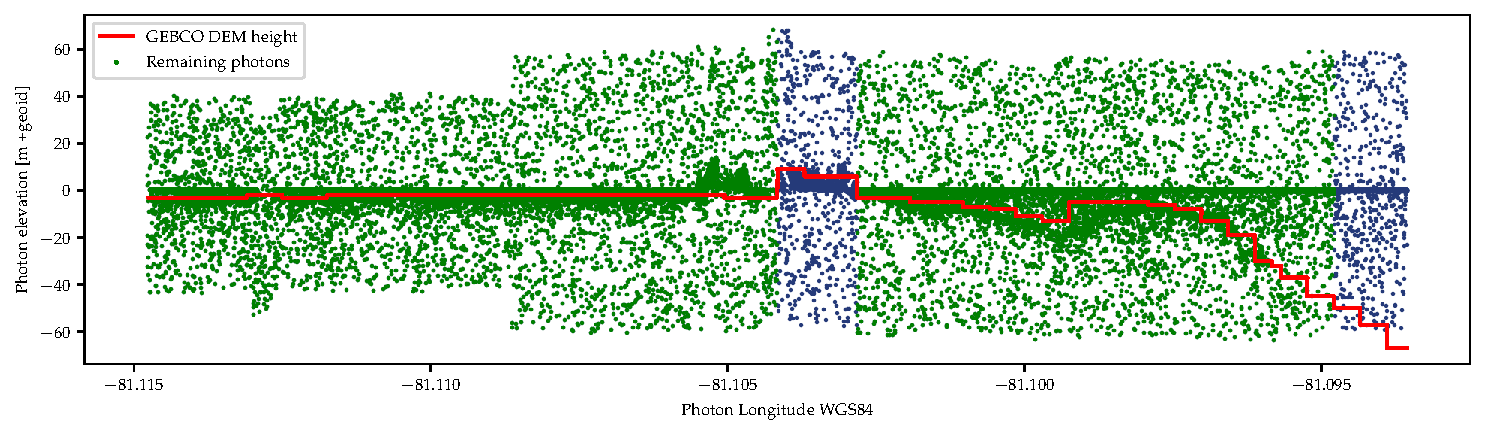
\includegraphics[width=\textwidth]{figures/methodology_gebco_filtering.pdf}
        \caption{The GEBCO data for the example transect, and the photons that are removed due to the GEBCO depth}
        \label{fig:gebco_filtering}
    \end{figure}

    \item To remove any high noise, cloud returns, or any remaining high land points not removed in step 1, any points more than 5m above the geoid are removed, based on the approach in \citeauthor{Ranndal2021}.
    \item The local sea-surface elevation $h_{sea}$ is calculated by taking the median elevation of the  high-confidence sea surface photons in the transect. The water depth for each photon is then calculated. The standard deviation of the elevation high-confidence photons $\sigma_{h_{sea}}$ is also calculated to estimate the magnitude of the wave height at the time of the observation.
    \item Any points with a water depth greater than 40 meters, and points with a geoidal height  less than -40m are removed, based on the same assumption that they are too deep to be bathymetric points. 
    \item Any points that are higher than $h_{sea} + max(\sigma_{h_{sea}},1)$ are removed. 
    
    
    The results of steps 3-5 are shown in figure \ref{fig:vert_filtering}
    % TODO fix this graph legend
    \begin{figure}[h]
        \centering
        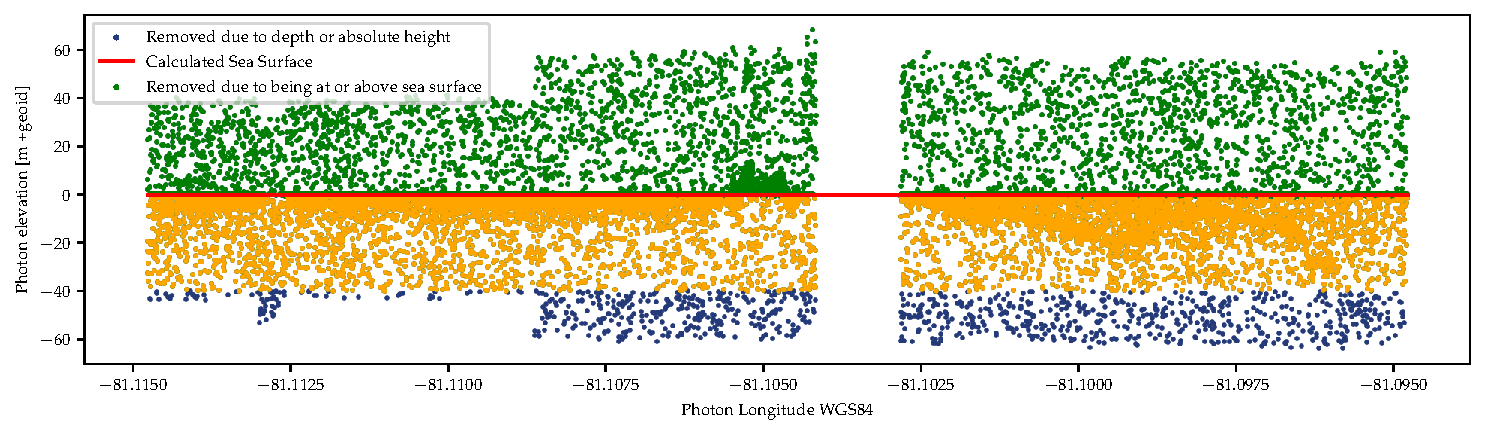
\includegraphics[width=\textwidth]{figures/methodology_sealvl_filtering.pdf}
        \caption{Vertical point filtering based on the local sea surface elevation}
        \label{fig:vert_filtering}
    \end{figure}
\end{enumerate}

After these filtering steps, the resulting subsurface photons for this example transect are shown in figure \ref{fig:remaing_photons}. The bathymetric signal can be seen clearly throughout the entire transect.

\begin{figure}[h]
    \centering
    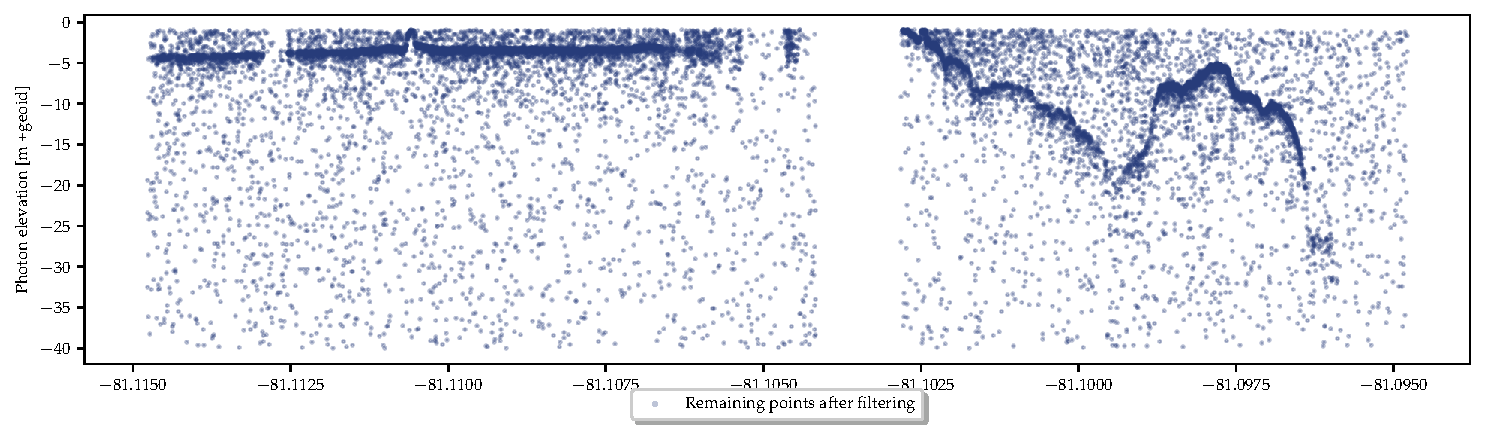
\includegraphics[width=\textwidth]{figures/methodology_reminaing_after_filtering.pdf}
    \caption{Subsurface photons found resulting after the filtering process}
    \label{fig:remaing_photons}
\end{figure}

An overview of the entire filtering chain is shown in figure \ref{fig:filtering-flowchart} \pdfcomment{mention checks for the number of filtered photons, and how it skips the transect if there are not enough photons}

\begin{figure}[h]
    \centering
    \import{figures/drawio}{Filtering_algo.drawio.svg.pdf_tex}
    % \import{figures/drawio}{filtering_v2.drawio.svg.pdf_tex}
    \caption{Filtering Process}\pdfcomment{figure out the word wrap issue}
    \label{fig:filtering-flowchart}
\end{figure}

Finally, before the signal-finding is applied, the Parrish method of refraction correction is applied to all subsurface photons.

\begin{figure}[htbp]
    \centering
    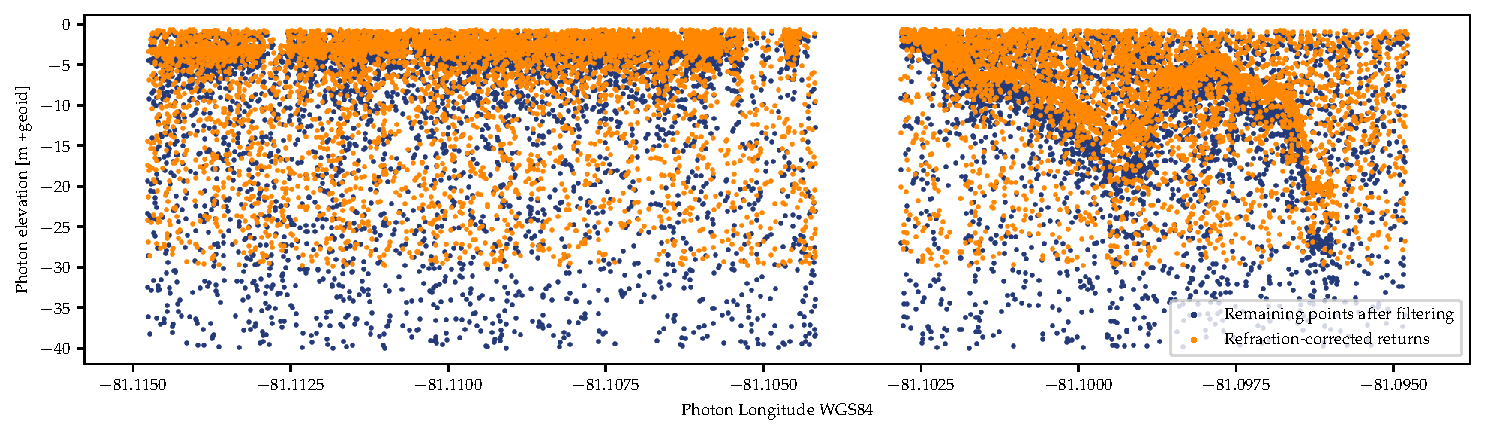
\includegraphics[width=\textwidth]{figures/methodology_refraction.pdf}
    \caption{The refraction correction applied to the remaining photons}
    \label{fig:refraction-photons}
\end{figure}

\subsection{Bathymetric Signal Extraction}\label{sec:kdesignalfinding}

The filtering steps reduce the dataset to just photon that are in the subsurface zone. To determine if there is bathymetric signal present, further processing is required. Some proposed methods for separating bathymetric signal photons from noise are explained in section \ref{subsec:denoising}. For this project, a new method is proposed based on a Gaussian Kernel Density Estimation (KDE) function. A function is created that returns the maximum kernel density, and the Z location at which it occurs. $$ f(\hat{z}_{window}) \rightarrow kde_{max},z_{kde_{max}} $$ Figure \ref{fig:kdefunc} shows the KDE function as applied to an example window, and the resulting kernel density plot. The KDE function is highly influenced by the \emph{bandwidth} parameter. For this implementation, the Scott method \parencite{Scott2015} is used to estimate the KDE bandwidth: $$ n^{\frac{-1}{d+4}} $$ where $n$ is the number of datapoints and $d$ is the number of dimensions of the data.

This function is applied on a rolling basis to a window of 100 adjacent photons. This function returns a value for every single point along the transect, including in areas that do not have any noticeable signal. The kernel density value gives an indication of the strength of the peak. To reject the locations where the signal is weak, any points with a KDE value of less than the median value $$ kde_{50} $$  are assigned an NaN value and are dropped from the analysis.

\begin{figure}[htbp]
    \centering
    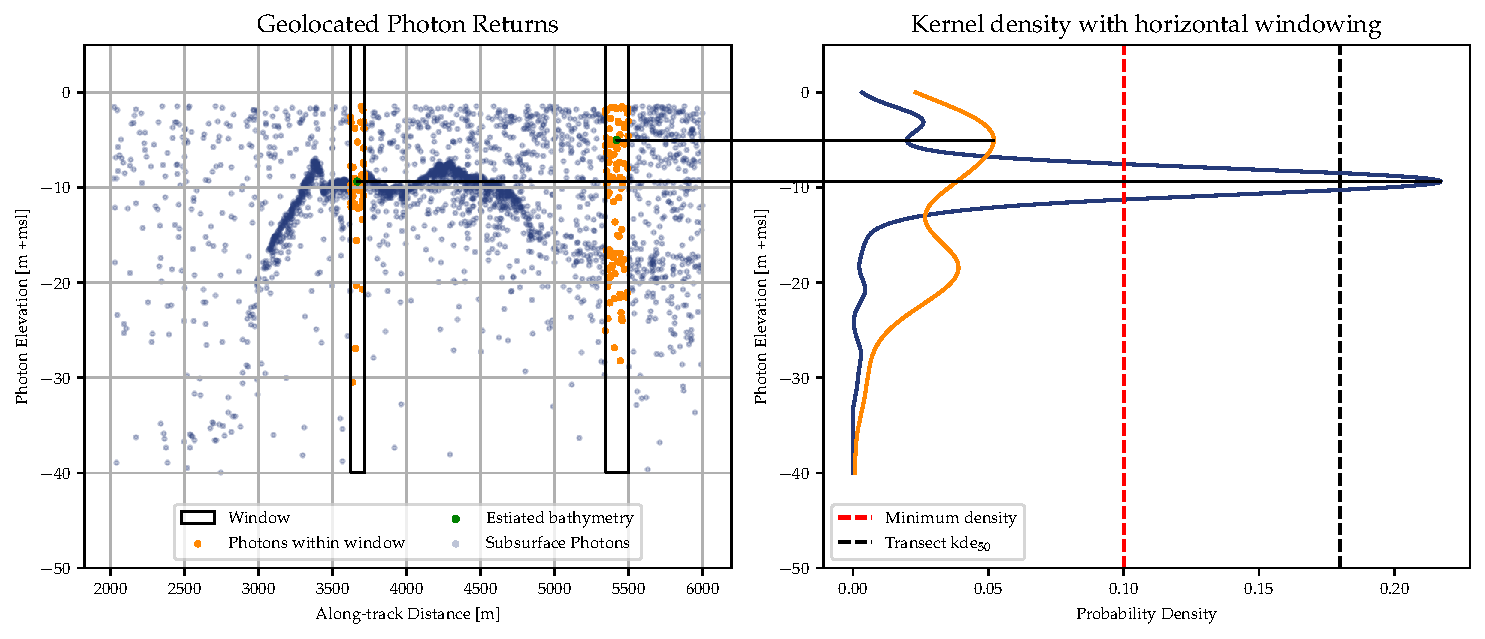
\includegraphics[width=\textwidth]{figures/2d_kde_plot.pdf}
    \caption{KDE function as applied to single window}
    \label{fig:kdefunc}
\end{figure}

The input parameters to the signal finding function are:

\begin{enumerate}
    \item The size of the window in \emph{number of points}
    \item the cutoff value for the Kernel Density required for point to be considered signal
\end{enumerate}

\subsection{Interpolation to a 2D grid}

After the bathymetric signal points are identified per the method in \ref{sec:kdesignalfinding}, the resulting bathymetry points are densely spaced along satellite tracklines, but are absent between them. A number of interpolation techniques have been applied to create bathymetry grids from point data. Commonly, inverse-distance weighting (IDW), tension splines, or loess interpolators have been used \parencite{gebcocookbook,Ferreira2017}. These approaches are relatively straightforward and easy to implement. However, the disadvantage of these simple approaches that there is not a clear methodology of establishing the uncertainty of the resulting interpolation. Intuitively, areas with a higher point density will lead to an interpolation with a lower uncertainty that areas with very sparse points. Kriging is a geostatistical technique that allows interpolating points into a grid, while also giving an indication of the uncertainty in the neighborhood. By knowing both our estimated sea floor depth and the uncertainty in the estimate, we can use a Bayesian approach to update our initial guess of the seafloor location.


\subsubsection{Subsampling of Bathymetric points using Poisson disk sampling} \pdfcomment{maybe add a figure to show the process better} \label{subsec:poissonsubsampling}
The bathymetric points are extremely densely spaced in some areas and transects. This can present an issue to kriging, which is computationally expensive and points too close together can make the algorithm even slower. To reduce the number of points fed into the algorithm, a subsample of the points is taken using the Poisson disk sampling technique. Poisson disk sampling is a strategy that generates random samples of a distribution that are a minimum distance apart. When applied to a point cloud, in this case the point cloud of all the bathymetric points, the sampling function will only return points that are a minimum distance apart in 3d space. This ensures that the sampling is as representative as possible of the underlying surface.

The implementation used is from the PDAL software library \parencite{howard_butler_2022_6369164}, which provides an iterative Poisson disk sampling function based on \citeauthor{McCool1992} (\citeyear{McCool1992}). The disk sampling is applied iteratively with a decreasing radius until the desired number of points is reached. In this case, it was found that the maximum number of points that can be practically be used in the kriging step approximately 2000 points. Therefore, this was the number of points used to allow the maximum possible point density while using consumer-grade laptops to run the algorithm. 

\subsubsection{Kriging interpolation}
Using the subsample of the points from the poisson disk sampling, they are converted to a bathymetry raster using universal kriging. This geostatistical technique results in both a raster of the estimated depth as well as the estimated uncertainty. The python package Pykrige \parencite{benjamin_murphy_2021_5380342} was used to implement the universal kriging approach. 

The univeral kriging interpolator used is a 2D interpolator, and both the estimated surface and its associated uncertainty are generatored for the entire site. A single slice of the output, taken along a icesat-2 transect, is shown in Figure \ref{fig:kriging-interpolator}. Note that the uncertainty estimate for the interpolated GEBCO surface is constant, and the uncertainty estimate for the kriging interpolator increases with increased distance from the measurement points. 

{fig:kriging-interpolator}
\begin{figure}[h]
    \centering
    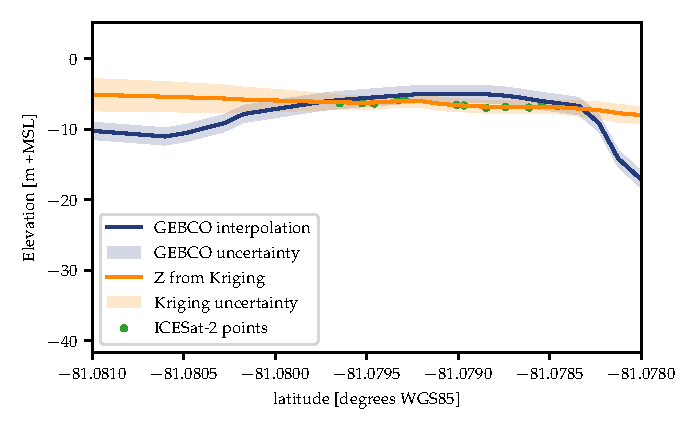
\includegraphics[]{figures/methodology-kriging-output.pdf}
    \caption{Example of the subsampled points, and the results of a kriging interpolation. In blue, the result of GEBCO is shown for comparison.}
    \label{fig:kriging-interpolator}
\end{figure}

\pdfcomment{add variogram parameter discussion}


\subsection{Bayesian data assimilation using Kalman update equation}
The Kalman Filter is a mathematical technique to predict the state of systems based on uncertain measurements. It consists of a loop of two steps, an \emph{time update} step which updates the position based on a measurement and a known measurement uncertainty, and a \emph{measurement update} step which predicts the state based on the dynamic equations of the system. The Kalman filter equations, is used to estimate the state of a linear process for a state $x_k$ and a vector of measurements of the state $z_k$ \parencite{Welch2021a}.  It is assumed that the state of a system evolves according to the difference equation

\begin{equation}
 x_k = Ax_{k-1} + Bu_{k-1} + w_{k-1}   
\end{equation}

Where $A$ is a matrix that relates the state at time step $k$ to the state at the previous time step and $w_k$ represents normally distributed process noise with a variance $Q$.  

Measurements of the state are assumed to have the form

\begin{equation}
    z_k = Hx_k + v_k
\end{equation}

Where $H$ is a matrix that relates the state to the measurement, and  $v_k$ is measurement noise which is assumed to be normally distributed with a variance $R$.

At each time step $k$, the estimates of the state can be updated according to the following two steps:

Time Update:
\begin{equation}\label{eq:timeup1}
    \hat{x}_{\bar{k}} = A\hat{x}_{k-1} + B\hat{u}_{k-1}
\end{equation}

\begin{equation}\label{eq:timeup2}
    P_{\bar{k}} = A P_{k-1} A^T + Q
\end{equation}

Measurement Update:
\begin{equation}\label{eq:kalmangain}
    K = P_{\bar{k}} H^T(H P_{\bar{k}} H^T + R) ^{-1}
\end{equation}

\begin{equation}\label{eq:new_state_measurement}
    \hat{x}_k = \hat{x}_{\bar{k}} + K(\hat{z}_k - H \hat{x}_{\bar{k}})
\end{equation}

\begin{equation}\label{eq:new_uncertainty}
    P_k = (I - KH)P_{\bar{k}}
\end{equation}

Where:
\begin{itemize}
    \item $\hat{x}_k$ is the current state of the system
    \item $\bar{k}$ is the measurement matrix
    \item $P_k$ is the error covariance matrix
    \item $K$ is the Kalman gain
\end{itemize}

To apply this to this bathymetry estimation problem, some simplifying assumptions are made. The nearshore zone is a highly dynamic system. However, for the purposes of this project is is assumed that the temporal variations over the time scale being studied are within the margin of error of the measurements, so the bathymetry of the nearshore zone is assumed to be a static system and the time update equations \ref{eq:timeup1} and \ref{eq:timeup2}. 

Equation \ref{eq:kalmangain} is the Kalman gain, an estimation of the strength of the estimation. For this case, it is assumed that the matrix $H$ is the identity matrix. Equations \ref{eq:kalmangain}, \ref{eq:new_state_measurement}, and \ref{eq:new_uncertainty} can be simplified to 

$$ K =  \frac{P_k}{P_k + R} $$

$$ \hat{x}_k =  \hat{x}_{\bar{k}} + K(\hat{z}_k -  \hat{x}_{\bar{k}}) $$


$$ P_k = (1 - K) P_{\bar{k}} $$


It is also assumed all measurements are measurements of the same underlying physical depth, and that differences between measurements are due to normally distributed measurement error, with magnitude of the error varying depending on the method. To combine multiple measurements, the \emph{measurement update} step is applied recursively for each available measurement, producing a Bayesian estimate of the bathymetry, in that it considers the uncertainty of each estimate. 

In this application, the starting point of estimate is based on a bilinear resampling of the GEBCO dataset, with an assumed variance of $1.5m^2$. Then, the simplified Kalman equations above are applied. At each raster grid cell the kriging uncertainty is used As $R$, and the kriged estimate of the seafloor is used as $\hat{z}_k$. The result is a new estimate of the bathymetry that includes both the kriged lidar surface and a priori depth of GEBCO. 

\begin{figure}[h]
    \centering
    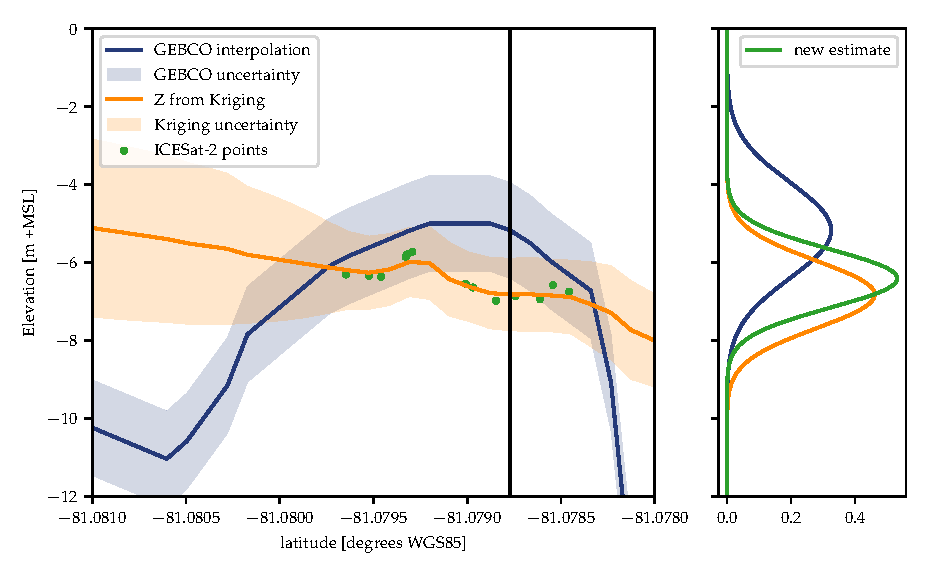
\includegraphics[width=\textwidth]{figures/methodology-kalman-updating.pdf}
    \caption{Using a section of the same transect in Figure \ref{fig:kriging-interpolater}, the processing of the Kalman measurement update is shown. }
    \label{fig:kalman-figure}
\end{figure}

\subsection{Per-track Secchi depth estimation}

The GlobColour Daily Secchi Depth dataset is provided at a 4km horizontal resolution, and a 1 day temporal resolution. To calculate the Secchi depth in water areas at the time of the satellite pass, the ATL03 tracklines divided into points every 4km starting at the end of the transect. Then, the GEBCO elevation at each point is found. Any points with a GEBCO elevation great than 0 are assumed to be over land, and are removed from the dataset. This works as a land mask to remove points occuring on land. The GlobColour dataset includes a land mask, but GEBCO has a much higher horizontal resolution than the GlobColour data ($~450m$ vs. $4km$, respectively). 

This provides a dataset of the ocean clarity (as estimated by Secchi Depth) data at the site \emph{on the day of the satellite pass.} Statistics can then be calculated for each unique trackline, or by each site as a whole.


\subsection{Error evaluation}

To validate the method, two different error metrics are considered. Both the error between the validation data and the lidar data is checked to evaluate the performance of ICESat-2 measurements, and the signal finding algorithm, and the total decrease in error between GEBCO and the version of GEBCO that includes the interpolated ICESat-2 data. 

The error metrics that are evaluated for both types of error are the root mean square error (RMSE) and the mean absolute error (MAE). The RMSE is calculated by taking the mean of the squared difference between the true value and the estimated value, and then taking the square root of this mean.

$$  RMSE = \sqrt{\frac{1}{n}\Sigma_{i=1}^{n}{\Big(\frac{d_i -f_i}{\sigma_i}\Big)^2}}  $$

By squaring the error first, larger magnitude errors are given relatively more weight in the metric. Mean absolute error also gives an idea of the average deviation, but gives equal weight to all errors.

$$ MAE = \sum_{i=1}^{D}|x_i-y_i| $$

To evaluate these errors between the Kalman-updated bathymetry grid and the validation data reprojection and resampling is required. The validation data has a horizontal resolution on the order of 1m, while GEBCO has a horizontal resolution on the order of 450m. Before taking the error, the data being compared is first reprojected into the native coordinate system and resolution of the validation data using GDAL \parencite{rouault_even_2022_6352176}. Then, the RMSE and MAE can be calculated between each cell of the raster grid.

\pdfcomment{make add figures showing the grid resampling/reprojection steps}

% \subsection{Evaluating transect-level variables which predict bathymetry}
% \pdfcomment{This could potentially be interesting and also help flesh out my answer to my first research question}
% \citeauthor{Hsu2021} found RMSE 0.26-0.61m, but they only had two transects.
% \pdfcomment{finish section}

\section{Possible limitations}

The starting point of this method is the level 2A product ATL03 data from NASA. It consists of raw photon locations and data about the atmospheric and geophysical parameters. 

\subsection{Limitations in Photon Geolocation Accuracy}

The pointing determination algorithm used by the satellite has a high vertical accuracy, but there is an inherent limitation on the horizontal accuracy. The current best estimate of the vertical accuracy is 0.17cm, and the estimate of the x and y position uncertainty is 5m \parencite{Neumann2019c}.

This uncertainty, and the horizontal refraction, are more likely second order effects. Because the kriging is used to create a product of 50m resolution, any uncertainty introduced by this will be masked by the interpolation to a 50m grid.

\subsection{Errors in refraction correction}

The refraction correction method used accounts for the additional horizontal error that is introduced by off-pointing. However, there are several other second-order effects that are not considered by the methodology. One of these is the estimation of the refractive index; the temperature and salinity affect the speed at which the water transmits light. By assuming a default value it introduces an error on the order of X.XXm \pdfcomment{Look this up to plug in some numbers to the formula to check}. This could be corrected by either estimating in advance a value for each local site, or by connecting the algorithm to an API that can provide a temperature and salinity value. 

Another potential source of error is the slope of the water surface. Since there is a slope to the water surface, this affects the bounce angle of the photon. This can be corrected for and some papers that investigate ICESat-2 bathymetry have attempted to correct for it. For this project the magnitude of error due to slope was considered small enough to be within the margin of error of the method.

\subsection*{Misclassified photons in ATL03 data}

Correcting filtering of sea surface returns is very important to the accuracy of the bathymetry signal finding, because the sea surface signal is often several orders of magnitude more dense than the bathymetric signal, and the location of the sea surface is also used to calculate the depth of a photon for refraction correction. The default photon classification provided in the ATL03 data is used to identify the sea surface within the filtering algorithm. Errors in the default ocean signal classification can result in sea surface signal being inadvertently included in the subsurface data and biasing the KDE results.

The default classification is often reliable, but when there is a large area where the bathymetric surface is shallow and nearly parallel to the sea surface, there can be misclassifications. An example of this is shown in figure \ref{fig:ageeba_bad_classes}. In this example, actual sea surface is not classified as a high confidence ocean surface return, and some areas that appear to be bathymetric signal are classified as ocean surface. This causes the bathymetric signal to be thrown out because it is incorrectly considered to be the sea surface.

This could potentially be mitigated by a different filtering strategy calculates the local sea surface based on the local geoid  This could be very feasible in microtidal areas where the tidal signal has a smaller impacts.

\pdfcomment{temp figure, replace with matplotlib figure with axis labels. Maybe also include a plan view map with scale bar to understand the geographic context}
\begin{figure}[htbp]
    \centering
    \includegraphics[width=\textwidth]{figures/ageeba_beach_example.png}
    \caption{Classification of photons from 2021-07-19, Beam gt3r, reference ground track 396. The two parallel straight lines from 200 to 800 are the sea surface and the bathymetric signal. The NASA photon classification algorithm misclassifies the bathymetric points as ocean surface returns}
    \label{fig:ageeba_bad_classes}
\end{figure}


\subsection{Limited spatial coverage in some islands}

In support of the vegetation mission of ICESat-2, the instrument is sometimes pointed up to several degrees to the side of the reference ground tracks when the satellite passes over land. This increases the spatial density of points at the expense of the temporal resolution. For bathymetric purposes the increased spatial resolution gives a more even  coverage of nearshore zone bathymetry. 

However, the land mask that is used to determine the off-pointing strategy has a limited resolution, and therefore some island nations do not benefit from the increased spatial density. This was noted when trying to collect data from Fiji and the Maldives. Due to apparently being located within the off-pointing zones, both of the aforementioned islands only have tracks which are 3km apart. They can still potentially collect bathymetry data if conditions are otherwise good, but the further reduction in spatial coverage limits the accuracy of the kriging method. This is unfortunate because many of the states that are at the highest need of detailed bathymetry for numerical studies are big ocean island nations. The tradeoff for this scenario is that the temporal resolution is significantly better, so the spaceborne lidar could be useful for studying the changes over time. 

\subsection{Inherent uncertainty of KDE Method}
There are a number of input parameters to the filtering and the density-based bathymetry finding methods. These parameters can be optimized for each site to reduce the RMSE error as much as possible if there is some validation data available. However since the end goal of the project is to be able to improve estimates without using any in situ data, ideally there would be no need for optimization based on the site.

Currently the globally-set parameters are sufficient to extract bathymetry without any tuning for all of the case studies that are investigated. However, the inability to tune in advance is a limitation. 

One possible future step would be to gather even more validation sites, and explore which other variables might influence the best parameter setting. It is possible that there are certain site variables which predict the optimal parameter options. Even so, upscaling of validation sites would allow better insight into which variables predict the presence of valid data.  

\subsection{ATL03 data quality issues}\label{sec:discussion-photon-issues}

There are a number of known issues with the ICESat-2 data. They are either due to atmospheric and environmental conditions, or due to limitations of the instrument. Many of them can be detected in advance, and then the effected granule data can be thrown out or the issue otherwise corrected for. However, there might be some edge cases related to these issues that cause either false bathymetric signal points, or cause the algorithm to miss valid bathymetric data. These data issues could present an issue for the scaling up the signal finding without any manual intervention. Currently the process is run without any intervention, but the sites are small enough to manually check several of the transects.

The following known data issues could effect the results of the KDE signal finding algorithm:

\subsubsection{Clouds}

The presence of some clouds along a single granule can cause the loss of data that might otherwise be valid

Clouds reflect sunlight which causes a higher background photon rate, and this can create issues with the telemetry bands and cause the telemetry bands to not include the surface. Even if the actual earth surface is included in the telemetry band, the clouds can affect the travel times and create inaccurate readings \parencite{atl03knownissues}.

During processing from L0 to L1, if the elevation from NASA reference DEM is not within the telemetry bands, no photons will be classified as signal. Therefore, if the entire granule is affected by this issue, there will be no sea surface found and therefore the entire granule will be filtered out. This can cause a significant loss of data but it is an issue inherent to nearly any remote-sensing based approach. One possible way to mitigate this would be to combine the ICESat-2 bathymetry data with synthetic aperture radar (SAR) remote sensing data. SAR remote sensing data can penetrate clouds because it uses radiometry outside of the visible spectrum. Although the spectrum used in SAR sensing cannot directly penetrate even clear water, the data can be used to estimate wave conditions, and the bathymetry can be estimated based on the transformation of the wave (called \emph{wave kinematic satellite-derived bathymetry}). The bathymetry estimates from SAR-derived wave kinematic SDB could be incorporated into the Kalman filtering step. 

In situations where the photons are able to pass through clouds, the changes to travel time through the clouds can affect the accuracy. This could potentially be something that is hard to detect and affect the accuracy of the bathymetric points if any are found.
 

\subsubsection{Multiple Telemetry Bands}

If the signal detection on board the satellite cannot determine where the primary surface is located, it will open another telemetry band to try to collect more signal. This can create other areas of photons that are significantly above or below the surface. The effect of is shown in figure \ref{fig:multiple_tel_bands}


\chapter{Results}


\pdfcomment{Compare the effect of other physical or atmospheric variables on the error, like include an entire section}
\pdfcomment{Add a point density per sqaure meter for each site}
\pdfcomment{average depth for each site?}

% \section{Random Sampling vs sampling along lines}

\section{Petten Test Site}
Most research results show that spaceborne lidar is not effective at retrieving bathymetry from very turbid waters. To test the upper limits of this, ICESat-2 data for the coast of Petten, NL was downloaded. As expected, there was no bathymetric signal found, likely due to the inability of the laser to penetrate the turbid water.

However, The Dutch government provides a dataset of point surveys of the Dutch coast. This data was used as input to the kriging and Kalman updating code.

\subsection{Site Conditions Summary}
\begin{table}[h]
    \begin{minipage}{0.5\textwidth}
        \centering\begin{tabular}{r l }
            Parameter                                                 & \textbf{Value}                  \\
            \hline
            Location                                                  &                                 \\
            Tidal Range \footcite{Tidal_data_reanalysis2022}          & \qty{2.24}{m}                   \\
            Average Secchi Depth \footcite{ACRI-STGlobColourTeam2020} & \qty{3.86}{m}                   \\
            Validation Data vertical RMS error                        & \qty{}{m} \pdfcomment{look up}  \\
            Validation Data Horizontal Resolution                     & \qty{}{m} \pdfcomment{look up?} \\
            Vertical Datum                                            & Normaal Amsterdams Peil (NAP)   \\
        \end{tabular}
    \end{minipage}
    \caption{Site conditions for the Florida Keys site}
    \label{table:Pettensitestats}
\end{table}

\subsection{Validation data}
The validation data for this site was from a 2021 survey performed by Van Oord.
\subsection{Error Jarkus Vs. Survey}
There was some error between the Jarkus survey points and the Van Oord 1m surveyed grid. The error metrics are shown in table \ref{tab:jarkus_vs_survey_error}, and the distribution of the error is shown in figure
\begin{table}[h!]
\caption{Error between Surveyed Bathymetry grid and Jarkus}
\label{tab:jarkus_vs_survey_error}
\begin{tabular}{lrr}
\toprule
 & MAE & RMSE \\
\midrule
Petten & 0.267152 & 0.439663 \\
\bottomrule
\end{tabular}
\end{table}


\begin{figure}[h]
    \centering
    \includegraphics[width=0.5\textwidth]{figures/Petten_lidar_estimated_vs_truth.jpg}
    \caption{Jarkus Survey points vs same location on Van Oord Survey data}
    \label{fig:jarkus_vs_survey}
\end{figure}

\subsection{Jarkus Data kriging and kalman Update}
\begin{table}[h!]
\caption{Improvement in Error when incorporating Kriged Jarkus data}
\label{tab:jarkus_kriging_kalman_error}
\begin{tabular}{lrr}
\toprule
 & RMSE & MAE \\
\midrule
Naive Bilinear Interpolation & 1.473726 & 1.311282 \\
Kalman Updated Raster & 0.722669 & 0.483035 \\
Kriged Raster & 0.743263 & 0.496904 \\
\bottomrule
\end{tabular}
\end{table}



\section{Marathon Key Test Site}
The area surrounding Marathon Key in the Florida Keys in Florida, USA. The area has a wide shelf, a microtidal tidal environment, and very clear water, so it is an ideal site to apply this methodolgy. 

\begin{table}[h]
    \begin{minipage}{0.5\textwidth}
        \centering\begin{tabular}{r l }
            Parameter                                                      & \textbf{Value}                                 \\
            \hline
            Location                                                       & -81.04472,24.72868                             \\
            Tidal Range \footcite{Tidal_data_reanalysis2022}               & \qty{0.51}{m}                                  \\
            Average Secchi Depth \footcite{ACRI-STGlobColourTeam2020}      & \qty{0.0}{m}                                   \\
            Validation Data Vertical RMS error \footcite{Keys2019Lidar}    & \qty{0.056}{m}                                 \\
            Validation Data Horizontal Resolution \footcite{Keys2019Lidar} & \qty{9.4e-6}{ \degree} $\approx$ \qty{0.95}{m} \\
            Vertical Datum \footcite{Keys2019Lidar}                        & local MSL                                      \\
        \end{tabular}
    \end{minipage}
    \caption{Site conditions for the Florida Keys site}
    \label{table:floridasitestats}
\end{table}


\subsection{ICESat-2 Transects within AOI}
The AOI used the validate the method is shown in figure \ref{fig:keys_transects} below.
\begin{figure}[h]
    \centering
    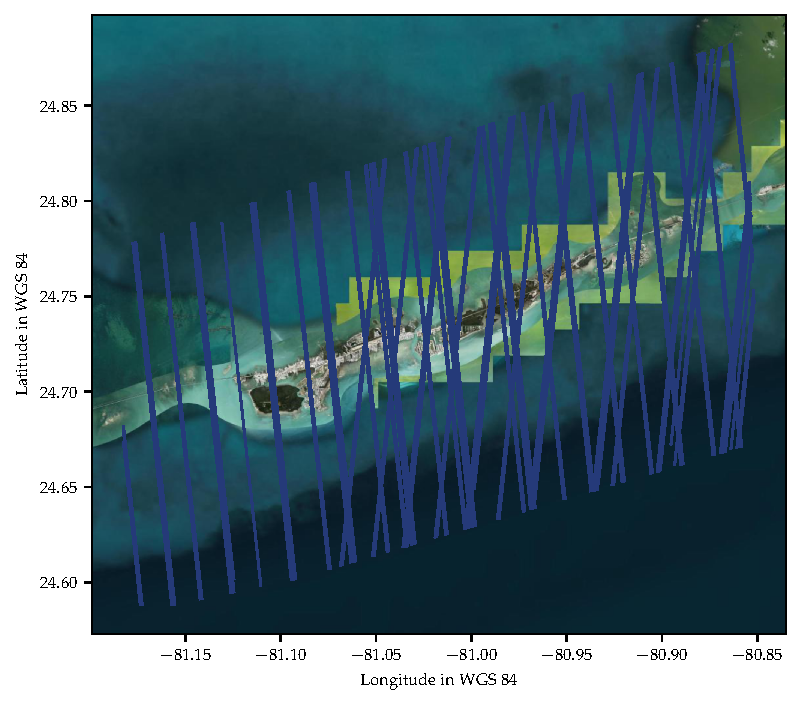
\includegraphics[width=0.5\textwidth]{figures/florida_keys_tracklines.pdf}
    % \input{figures/study_site_tracklines.pgf}
    \caption{Location of ICESat-2 Transects in Florida keys Study Area}
    \label{fig:keys_transects}
\end{figure}
\subsection{Validation Data}
The validation data used for this site is from a detailed lidar survey of the area performed in 2018 and 2019 by Quantum Spatial, Inc. \parencite{Keys2019Lidar}. The survey was performed using a Riegl VQ-880-G hydrographic airborne laser scanner. The instrument is designed for high bathymetric accuracy in shallow water.
%removing validation data for now, maybe replace this with a contour map 
% \begin{figure}[h]
%     \centering
%     \includegraphics[width=\textwidth]{figures/florida_keys_ras.jpg}
%     \caption{Ground Truth topobathymetric Survey taken after Hurricane Irma}
%     \label{fig:truebathy}
% \end{figure}
\subsection{Error in lidar photon data}
After extracting the bathymetry from the ICESat-2 transects over the study site, the RMS error between the measured data from the USGS and the ICESat-2 data is
\begin{figure}[h]
    \centering
    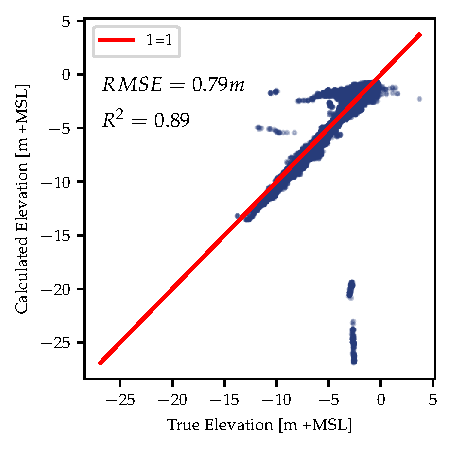
\includegraphics[width=0.5\textwidth]{figures/florida_keys_lidar_estimated_vs_truth.pdf}
    \caption{Comparison between depth calculated with ICESat-2 and true bathy}
    \label{fig:fl_truth_vs_measured_points}
\end{figure}
% \begin{table}
\caption{Atmospheric Profile vs error}
\begin{tabular}{lr}
 & 0 \\
atm_profile &  \\
profile_1 & 0.524872 \\
profile_2 & 0.666805 \\
profile_3 & 0.551757 \\
\end{tabular}
\end{table}


% \begin{table}
\caption{Beam Strength vs Error}
\begin{tabular}{lr}
 & RMS error \\
beamtype &  \\
strong & 11.206860 \\
weak & 9.363623 \\
\end{tabular}
\end{table}


\subsection{Bathymetric photons}
Figure \ref{fig:bathyphotonmap} shows the location and estimated bathymetric depths of individual ICESat-2 photon returns.
\pdfcomment{change colorbars to match}
\begin{figure}[h]
    \centering
    \includegraphics[width=\textwidth]{figures/Florida_keys_photon_map.pdf}
    \caption{Geographic distribution of Bathymetric photon data}
    \label{fig:bathyphotonmap}
\end{figure}

\subsection{Lidar updated GEBCO vs. Simple bilinear Interpolation}
The results when comparing a raw interpolation of GEBCO to
% \begin{table}[h!]
\caption{Comparison of the error metrics between the Kalman updating and a simple bilinear interpolaton of GEBCO data}
\label{raster_rmse_comparison}
\begin{tabular}{lrr}
\toprule
 & RMSE & MAE \\
\midrule
Naive Bilinear Interpolation & 2.086102 & 0.986900 \\
Kalman Updated Raster & 1.345899 & 0.836557 \\
\bottomrule
\end{tabular}
\end{table}

\begin{table}
\centering
\caption{Improvement in error metrics after applying Kalman Updating of kriged data}
\label{tab:florida_keys_gebco_raster_error}
\begin{tabular}{lrr}
\toprule
 & RMSE & MAE \\
\midrule
Naive Bilinear Interpolation & 2.21 & 1.11 \\
Kalman Updated Raster & 1.41 & 0.85 \\
Kriged Raster & 2.28 & 1.31 \\
\bottomrule
\end{tabular}
\end{table}



\section{St. Croix}

\subsection{Site Characteristics}

St. Croix is in the US Virgin Islands. \pdfcomment{flesh out}

\begin{figure}[h]
    \centering
    \includegraphics[width=\textwidth]{figures/Stcroix_tracklines.pdf}
    \caption{Tracklines in the St. Croix site}
    \label{fig:st-croix-tracklines}
\end{figure}

\subsection{ICESat-2 Signal Extraction}
After downloading the above tracklines and processing them, the points shown in were identified by the algorithm as containing bathymetric measurements.

\begin{figure}[h]
    \centering
    \includegraphics[width=\textwidth]{figures/Stcroix_photon_map.pdf}
    \caption{Point estimates of bathymetry from KDE algorithm }
    \label{fig:stcroix-bathy-points}
\end{figure}

This site showed excellent agreement between the point ICESat-2 estimated lidar and the validaton data. The error metrics are shown in table

\begin{table}[h!]
\caption{Error between the point bathymetry and ground-truth data}
\label{tab:stcroix_lidar_error}
\begin{tabular}{lrrrrr}
\toprule
 & MAE & RMSE & Median Abs error & R2 Score & Average Error \\
\midrule
stcroix & 0.299882 & 0.545965 & 0.176959 & 0.975837 & -0.087435 \\
\bottomrule
\end{tabular}
\end{table}


\subsection{Gebco Updating}

The improvement in error is shown in table ref{tab:stcroix-raster-error}

\begin{table}
\centering
\caption{Improvement in error metrics after applying Kalman Updating of kriged data}
\label{tab:stcroix_gebco_raster_error}
\begin{tabular}{lrrr}
\toprule
 & RMSE [m] & MAE [m] & Mean Error [m] \\
\midrule
Naive Bilinear Interpolation & 6.45 & 4.30 & -1.01 \\
Kriged Raster & 6.79 & 4.10 & -2.91 \\
Kalman Updated Raster & 4.63 & 3.20 & -1.14 \\
\bottomrule
\end{tabular}
\end{table}


\section{Charlotte Amalie}
Another test site is the island of Charlotte Amalie in the US Virgin Islands. Basic details about the test site are in \ref{table:charlotteamalie_datatable}
\begin{table}[h]
    \begin{minipage}{0.5\textwidth}\pdfcomment{fill in table}
        \centering\begin{tabular}{r l }
            Parameter                                                 & \textbf{Value} \\
            \hline
            Location                                                  &                \\
            Tidal Range \footcite{Tidal_data_reanalysis2022}          & \qty{}{m}      \\
            Average Secchi Depth \footcite{ACRI-STGlobColourTeam2020} & \qty{}{m}      \\
            Validation Data vertical 95\% confidence                  & $x$ m          \\
            Validation Data Horizontal Resolution                     & \qty{}{m}      \\
            Vertical Datum                                            & lookup         \\
        \end{tabular}
    \end{minipage}
    \caption{Site conditions for the Charlotte Amalie}
    \label{table:charlotteamalie_datatable}
\end{table}
Overall there where X \pdfcomment{lookup number of transects} transects of ICESat-2 data available for the site, and their distribution is shown in figure \ref{fig:charlotteamalietracklines}.

\begin{figure}[h]
    \centering
    \includegraphics[width=\textwidth]{figures/Charlotteamalie_tracklines.pdf}
    \caption{ICESat-2 tracks in the Charlotte Amalie Test site}
    \label{fig:charlotteamalietracklines}
\end{figure}

\subsection{Lidar Points found for site}
Figure \ref{fig:pointmapcharlotteamalie} shows the geographic distribution of the points

\begin{figure}[h]
    \centering
    \includegraphics[width=\textwidth]{figures/Charlotteamalie_photon_map.pdf}
    \caption{Charlotte Amalie points}
    \label{fig:pointmapcharlotteamalie}
\end{figure}

The error for the site is shown in \ref{fig:charlotteamalie-lidar-bias}

\begin{figure}[h]
    \centering
    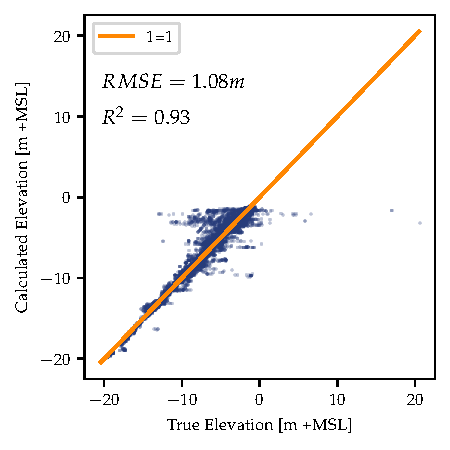
\includegraphics[width=0.5\textwidth]{figures/charlotteamalie_lidar_estimated_vs_truth.pdf}
    \caption{Bias plot showing the agreement between the validation data and the lidar points for Charlotte Amalie}
    \label{fig:charlotteamalie-lidar-bias}
\end{figure}


\section{Oahu}
One test site that was selected based on the clear water and the high quality validation data is the Island of Oahu, in the US state of Hawai'i. The island has an extremely varied shelf and coastal environment along its length, to it provides the ability to test the results in in areas with a variety of offshore slopes and wave energy environments.

Because of the size of the island, the nearshore zone was divided into 8 different zones, for which the data was downloaded and processed seperately. The results were then combined and summarized. A map of the area that shows the available ICESat-2 tracklines and the subareas used to download the and process the data are shown in figure \ref{fig:oahu-all-sites-transects}

\begin{figure}[h]
    \centering
    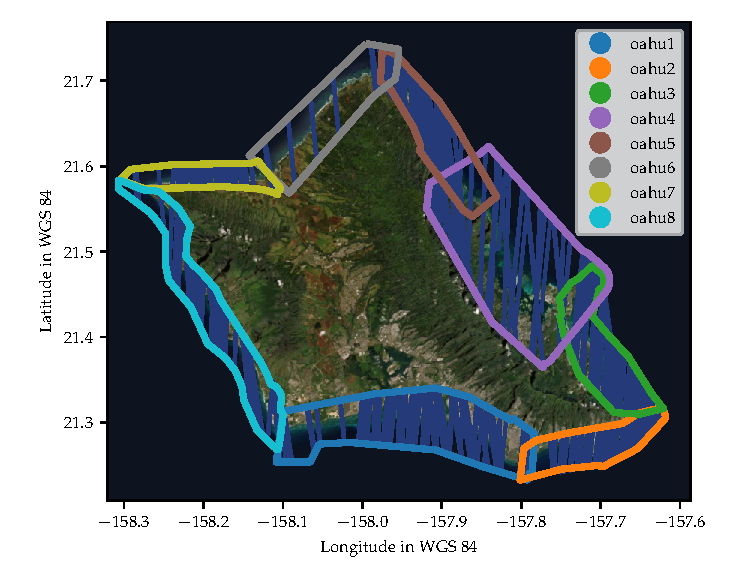
\includegraphics[width=\textwidth]{figures/Oahu_all_tracklines.pdf}
    \caption{Transects and subsite distribution for Oahu Test site}
    \label{fig:oahu-all-sites-transects}
\end{figure}

\subsection{ICESat-2 Signal Extraction}

The data for all 8 subsites was downloaded and the filtering and KDE signal finding steps were applied. Figure \ref{fig:oahu-all-photon-map} shows the spatial distribution

\begin{figure}[h]
    \centering
    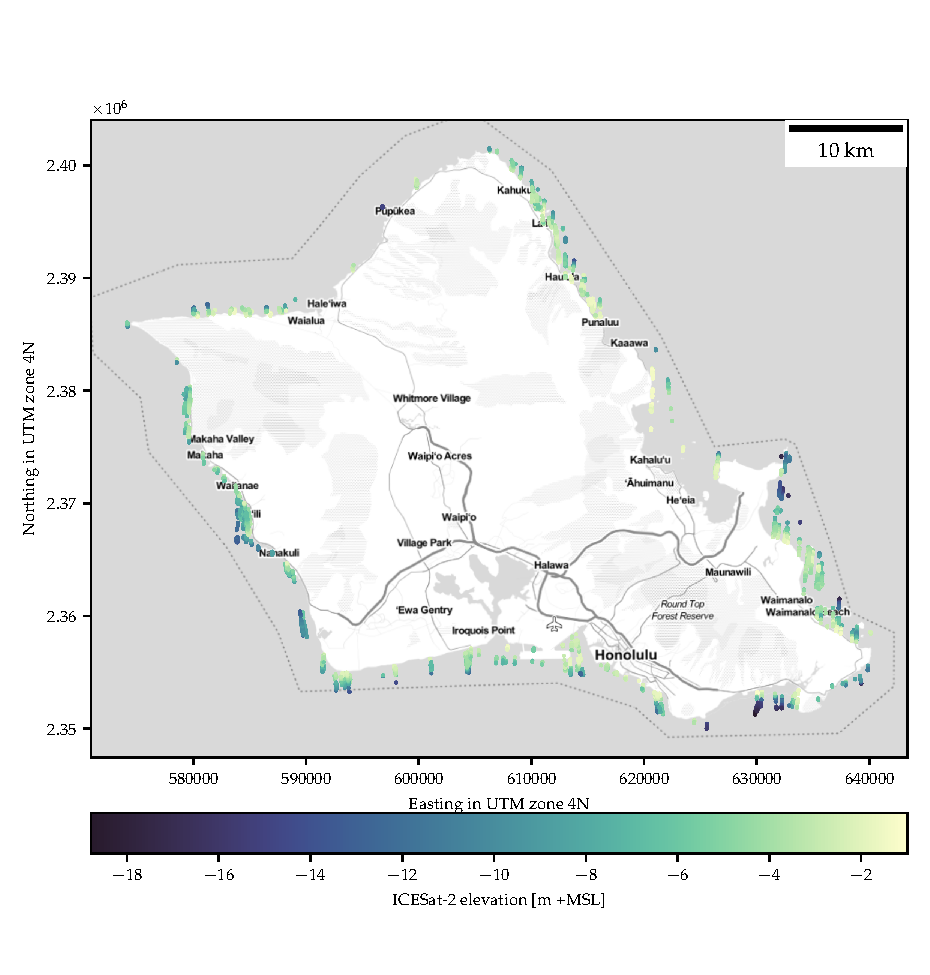
\includegraphics[width=\textwidth]{figures/Oahu_all_sites_photon_points.pdf}
    \caption{The layout of the identified bathymetry point measurements around Oahu}
    \label{fig:oahu-all-photon-map}
\end{figure}

The sites varied significantly in in the accuracy of the ICESat-2 point bathymetry. Some sites showed a significant RMS error due to the precense of mountain peaks up to a few hundred meters high with small horizontal footprint. These features are not captured by the GEBCO grid and therefore photon returns below them are not filtered due to the GEBCO-based horizontal filtering. Table \ref{table:Oahusitestats} contains the compiled error metrics for each site.

\pdfcomment{add to discussion section} \pdfcomment{good to explain with a figure I think}

\begin{table}[h!]
\caption{Error metrics between ICESat-2 and ground-truth data for all sites in Oahu}
\label{tab:Oahusitestats}
\begin{tabular}{lrrr}
\toprule
 & RMSE & MAE & Count bathy Points Identified \\
Oahu site number &  &  &  \\
\midrule
1 & 1.162525 & 0.768264 & 12775 \\
2 & 10.598899 & 1.447226 & 4327 \\
3 & 1.235144 & 0.463879 & 18566 \\
4 & 0.751631 & 0.565673 & 2738 \\
5 & 0.734813 & 0.504969 & 10443 \\
6 & 2.422447 & 1.756412 & 754 \\
7 & 1.111055 & 0.717672 & 2949 \\
8 & 0.670030 & 0.520755 & 17946 \\
\bottomrule
\end{tabular}
\end{table}


The overall bias plot showing all the subsites is shown in figure \ref{fig:oahu-all-bias-plot}

\begin{figure}[h]
    \centering
    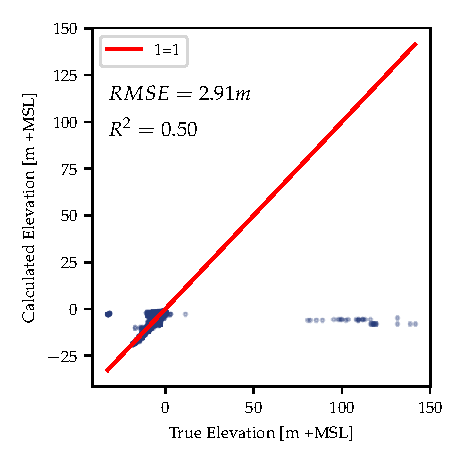
\includegraphics[width=0.7\textwidth]{figures/Oahu_combined_lidar_estimated_vs_truth.pdf}
    \caption{Bias plot for all Oahu subsites combined}
    \label{fig:oahu-all-bias-plot}
\end{figure}

The reason the RMSE at site 2 is much higher than the rest is that there was a mountain of 120m tall that was in the validation data. If that is removed, the error drops significantly. \pdfcomment{outlier rejection might be a fix for that.}
\pdfcomment{these two figures could be combined into subplots probably }
\begin{figure}[h]
    \centering
    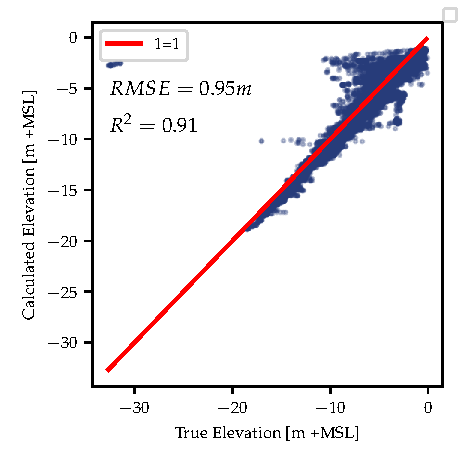
\includegraphics[width=0.7\textwidth]{figures/Oahu_combined_mountains_removed_lidar_estimated_vs_truth.pdf}
    \caption{Oahu - all sites with mountain removed}
    \label{fig:oahu-bias-no-mountains}
\end{figure}

To better show the distribution of the error smaller erros, figure \ref{fig:oahu-bias-no-mountains} shows the same combination of points, but with the outlier values 

\subsection{Kalman Updating}



\section{Summary}
The results of all the test sites that used lidar data were combined into a single bias plot shown in figure \ref{fig:all-sites-biasplot}

\subsection{ICESat-2 error}

\begin{figure}[h]
    \centering
    \includegraphics[width=0.7\textwidth]{figures/all_site_combined_biasplot.pdf}
    \caption{All lidar points for all sites with validation data}
    \label{fig:all-sites-biasplot}
\end{figure}


\chapter{Discussion}

\section{A-priori identification of transects with bathymetric signal}
One of the goals of the project is to find a way to predict nearshore zones which are most likely to have ICESat-2 bathymetry available before downloading the photon-level data and running the KDE signal finding algorithm. A-priori identification of promising sites is useful to minimize the computing resources required when scaling up the approach to a global level.

When looking at the transect data as a whole, there was no single variable which predicts either the availability or the quality (measured by RMSE) of bathymetric data contained in a given transect. It is well-established that lidar and optical bathymetry are highly sensitive to turbidity levels, since they require light to be able to reach the seafloor. It was hypothesized that the Secchi depth, as estimated by optical satellite methods, would be a reliable indicator of bathymetric quality and quantity for a given transect. However, no clear relationship was found between the Secchi depth and the quality and quantity of bathymetric signal photons. In fact, the Florida Keys test site has the lowest median Secchi depth (8.3 m) of any of the test sites investigated, while also providing some of the highest quality data (0.87 m RMSE), and the largest percent of transects containing valid signal of any test site. 

The most likely explanation for this seeming paradox is that the characteristics that make a site ideal for ICESat-2 bathymetry (i.e., a wide, shallow shelf with clear water) could affect the accuracy of optical ocean color measurements. The area of interest selected in the Florida Keys site has large areas with a depth of less than 10 m, and exceptionally clear water. The Secchi depth determination is based on passive optical remote sensing response of the site. It is possible that because in this site there is a very significant amount of sunlight reflecting from the seabed, the Secchi depth algorithms used in the GlobColour product have limited accuracy. This is further supported by the fact that the Secchi depth uncertainty metric (median 56\% uncertainty) is much higher for the Florida Keys site than any other site. Table \ref{tab:ocean_color_summary_by_site} shows the median Secchi depth and light diffusion coefficient for each subsite, as well as the RMSE and MAE error between the ICESat-2 point data and the validation data.


\begin{table}
    \centering
    \caption{Secchi Depth and RMSE for each site}
    \label{tab:ocean_color_summary_by_site}
    \begin{tabular}{lrrrrrr}
        \toprule
        {}
        Site Name           & $Zsd_{50}$[m] & $\sigma_{Zsd_{50}}$ & RMS Error [m] & MAE [m] & ME [m] \\
        \midrule
        St. Thomas/St. John & 23.52         & 23.92               & 1.08          & 0.56    & -0.17  \\
        Florida Keys        & 8.29          & 56.01               & 0.79          & 0.31    & 0.24   \\
        Oahu 1              & 29.70         & 29.52               & 1.16          & 0.77    & 0.54   \\
        Oahu 2              & 31.59         & 28.97               & 10.60         & 1.45    & 1.41   \\
        Oahu 3              & 28.43         & 50.92               & 1.24          & 0.46    & 0.30   \\
        Oahu 4              & 28.43         & 27.14               & 0.61          & 0.39    & 0.26   \\
        Oahu 5              & 29.84         & 25.48               & 0.73          & 0.50    & 0.27   \\
        Oahu 6              & 28.93         & 31.82               & 2.42          & 1.76    & -1.43  \\
        Oahu 7              & 32.76         & 25.54               & 1.11          & 0.72    & -0.02  \\
        Oahu 8              & 33.26         & 23.75               & 0.67          & 0.52    & 0.35   \\
        St. Croix           & 26.89         & 41.20               & 0.54          & 0.30    & -0.11  \\
        \bottomrule
    \end{tabular}
\end{table}


\section{Bathymetry extraction from ICESat-2 lidar}

Compared to other signal finding methods proposed in the literature, the implementation used here results in a similar order of RMSE for most of the test sites. The KDE signal finding method proposed was able to identify bathymetric photons with an RMSE of between 0.54 m and 9.53 m RMSE. This is a very wide range of reliability, and would require further refinement before scaling the method to more sites. The site with the largest error was in an area with steep cliffs on the south end of Oahu, Hawai'i. The source of the error was a failure in the horizontal filtering approach. The error was caused by some points with a true elevation of 118 m being labeled as subsurface photons. Because they are in a land area, they should have been removed by the GEBCO filtering step. However, because of the limited horizontal resolution of GEBCO data they were not removed from the photon cloud during subsurface photon filtering.

The best way to mitigate this would be to find a better land mask dataset. This is likely possible for sites in the global north that have good data availability, but higher resolution land masks might not be available in the entire world. It should be noted that the ATL03 dataset does include a surface mask flag as one of the variables. However, it is not suitable for this purpose because there is an intentional overlap between the boundaries of these different masks. Therefore, a photon return in a coastal zone can be classified as being both in the ocean, land, and inland water zones. This is done because it is assumed there is a high uncertainty in the exact boundaries between surface types. 

One of the challenges of the proposed KDE signal finding method is that it is very sensitive to the input parameters, especially the threshold KDE value to distinguish signal from noise. The threshold used here was set empirically, and it was the greater of either a.) the median KDE of the transect, or b.) 0.1. By making this criterion stricter (increasing the minimum to 0.15) the RMS error at each site can be reduced significantly. However, this presents a tradeoff. While a few large magnitude errors are filtered out by increasing this threshold, there are many times more high-quality points that are also excluded. This can be seen in Figure \ref{fig:zoomed-inset-error}, where the inset plot shows the relative density of low-error photons which have a KDE value less than 0.15. By excluding these points, it often reduces the overall spatial distribution of the resulting point data (the KDE is correlated for a given transect, so by increasing the threshold, often entire transects worth of points are removed). Therefore, increasing this threshold is quite a blunt instrument that removes significant amounts of high quality data. It was found that using a lower density threshold, and therefore allowing some large errors to remain in the point data, the overall quality of the kriging interpolation and the resulting Kalman-updated output product was improved. 

\begin{figure}[htbp]
    \centering
    \includegraphics[width=0.8\textwidth]{figures/threshold_discussion_inset.png}
    \caption[Effect of minimum density threshold parameter choice]{Effect of minimum density threshold parameter choice. The red line shows a threshold of 0.15. If this was used as the signal classification threshold, this removes almost all the most severe errors but also eliminates many times more high quality points, resulting in a tradeoff between the quantity and quality of points}
    \label{fig:zoomed-inset-error}
\end{figure}

One potential avenue for improving the discretion of the algorithm would be considering the local horizontal density of photon returns. A rolling window based on distance rather than a set number of adjacent photons could potentially improve the quality of the KDE magnitude estimation. Another approach might be to normalize the KDE value based on the transect length, and see if that improves the ability to throw out low-quality data while retaining high-quality data.

Another approach for discriminating between signal and noise photons could be to set a threshold based on the depth of the photon. In the bias plots of the lidar error for each site, the spread around the 1=1 line is greater for shallower parts of the nearshore zone. Because the attenuation of light energy increases with depth, one would normally expect less strong signal, and therefore lower accuracy, in deeper waters. However, this error could be an artifact of the KDE algorithm; sometimes photons are reflected in the first few meters of the water column, therefore the first few meters of the water column contain noise that is slightly biased toward the top of the water column. This noise is less dense than a seafloor return, but might sometimes be dense enough to reach the minimal density threshold and be misclassified as signal. 

It is possible that the results could be further improved by building a larger dataset of validation sites, and trying to find globally optimum parameters that provide a good balance of excluding low accuracy points and maintaining as much quality data as possible.

\section{2D interpolation via universal kriging}

The universal kriging approach proved effective to transform the point estimates into a gridded estimate of seabed elevation and uncertainty. 

The largest practical limitation to the Bayesian updating method is the requirement to interpolate the data. The Kriging interpolater is ideal because they are robust to outliers and provide an uncertainty estimate as well as a depth estimate. The downside of the kriging interpolator is both the computational complexity and the requirement that points are not too close together. If points are too close to one another, the kriging matrix is not soluble, and the algorithm has a complexity of $\mathcal{O}(n^4)$ where $n$ is the number of points being interpolated. This means that there is a relatively strict practical limitation to the number of points that can be used as input to the interpolator. The upper limit with a laptop with 32GB RAM was found to be approximately 2000 points without exceeding the available memory. One way to deal with this is to use a tiling strategy, and repeat the process using tiles which contain 2000 bathymetric points or less. This would need to be done adaptively since the bathymetric points are not evenly distributed. Using a larger number of smaller sub-sites would take longer to process, but it would at least be feasible using a consumer-grade computer.

One disadvantage of ICESat-2 data is the uneven spatial distribution of the resulting bathymetric points. Due to the orbit of ICESat-2, the ATL03 data is available along transects oriented $\pm \ang{6}$ relative to north (see Figure \ref{fig:distribution-of-bathy-points-in-space}). Because of this pattern, even if there was perfect bathymetry data along every single ICESat-2 transect within the study area, the spatial distribution of the points would be anisotropic. Given that there are gaps in these transects where the bathymetric signal is weaker, the spatial distribution of the data can vary significantly by site. An example of the gaps that can occur along transects can be seen in Figure \ref{fig:distribution-of-bathy-points-in-space}. The gaps of weaker signal can be caused by areas that are too deep or too turbid for the lidar photon to reach the seabed, or due to instrument/atmospheric issues (see sec. \ref{sec:discussion-photon-issues}). 


\begin{figure}
    \centering
    \includegraphics[width=0.9\textwidth]{figures/discussion-spatial-stcroix.pdf}
    \caption[Spatial distribution of bathymetry points in St.~Croix north end]{Spatial distribution of bathymetry points in St.~Croix north end, and the true bathymetry. The red lines show transects. The north end of the transects in this figure are cut off by the request polygon. The black dots show the locations of bathymetric signal as identified by the KDE signal finding algorithm.}
    \label{fig:distribution-of-bathy-points-in-space}
    %\pdfcomment{label colorbar, fix overfull hbox issue, north arrow and scale bar}
\end{figure}

However, handling this uneven spatial distribution is one of the advantages of using a geostatisical approach. Areas that are distant from any input points have a higher uncertainty in the output grid, and therefore there is little or no change from the prior estimate, since the Kalman update step accounts for the estimate uncertainty. Therefore, in locations that are further away from valid data, there is little or no change from the prior estimate. A limitation of this is that any accuracy gains are might not be evenly distributed across the site. 

\section{Kalman updating and improvement over GEBCO}

It was found that in most sites, the Bayesian combination of bilinearly resampled GEBCO data and the interpolated ICESat-2 data increased the accuracy compared to the validation data than either product on their own. The decrease in RMSE achieved was up to 34\% in some sites, but in other sites actually showed an increase. This could likely be mitigated by optimizing the assumptions behind the measurement uncertainties.

\begin{table}[htbp]
\centering
\caption[Summary of percent change in error metrics for each test site]{Percent reduction in error metrics via the Kalman updating approach. Positive values indicate reduced error, negative ones indicate increased error}
\label{tab:allsite-percent-change}
\begin{tabular}{lrrr}
\toprule
 
sitename & RMSE Change & MAE Change & ME Change \\
\midrule
Florida Keys & 34.41\% & 22.83\% & 456.68\% \\
St.~Croix & 28.15\% & 26.59\% & -4.74\% \\
St.~Thomas and St.~John & 21.41\% & 19.88\% & 194.37\% \\
Oahu 1 & 28.43\% & 30.75\% & 73.46\% \\
Oahu 2 & 31.62\% & 29.61\% & 51.10\% \\
Oahu 3 & 25.18\% & 22.68\% & 75.06\% \\
Oahu 4 & -1.76\% & -1.01\% & 123.78\% \\
Oahu 5 & 1.94\% & 4.52\% & 116.88\% \\
Oahu 6 & -18.14\% & -16.12\% & -14.68\% \\
Oahu 7 & -22.61\% & -15.04\% & -16.58\% \\
Oahu 8 & -25.15\% & -21.05\% & -544.94\% \\
\bottomrule
\end{tabular}
\end{table}


The optimal decrease in RMS error was found by assuming a GEBCO uncertainty of $\sigma=1.5~m$ standard deviation. This produced the best results for the test sites under consideration, however the actual GEBCO uncertainty depends on myriad factors including the original data source, survey method, and how old it is. One improvement that could be further explored is how the uncertainty of GEBCO varies with the Type IDentifier (TID) grid. The TID is a GEBCO data product that indicates the original source of the data. It is likely that the original data source affects the error between the GEBCO grid and the validation data.

One limitation is that the temporal resolution of the ICESat-2 data is not sufficient to take full advantage of the Kalman filtering approach, which normally includes updates both in space and time. The satellite repeat time for a given reference ground track is 91 days, and the data is available starting in 2018. Due to off-pointing over most land areas, there is often greater than 91 days between passes of the \emph{exact same} track. Since coasts are among the most dynamic morphological environments, there might be substantial changes between repeat passes. The proposed method assumes that all ICESat-2 bathymetry data is contemporaneous. This is an inherent limitation to the method, since it cannot account for morphological changes that might occur during the 4-year time window in which the data was collected. However, the ICESat-2 data is very likely more recent than the input data to the GEBCO gridding process, which in some places can come from digitized nautical maps that can be hundreds of years old. Therefore, all data was assumed to be contemporaneous, and the time update step of the Kalman Filter was not used.

One potential downside of the Bayesian update approach is that it could create artifacts in the resulting output data, even if the RMS error is decreased relative to GEBCO. If there is an area with a high density of poor quality point measurements, the resulting uncertainty data might have a high confidence in that local area, leading to a significant update to the prior estimate which does not reflect a physical seabed  feature. This effect could create artificial shoals or shallow areas. \pdfcomment{this probably needs a graphic to help explain} Because the RMS error is decreasing relative to the validation data, we know that the \emph{net} effect of the Bayesian update is an improvement. However, the addition of phantom shoals could make the unsuitable for numerical modeling studies, since introducing an artificial high point offshore could change the wave transformation results significantly. However, the decreased average error of the downscaled product could have utility for estimating dredging quantities, which are less sensitive to an individual high point. 
\chapter{Conclusions}
This section summarizes the findings after implementing the toolchain as described in section \ref{sec:methodology} as described.

\section{Research Question}
To answer the primary research question \emph{How can spaceborne remote sensing data be combined with existing global datasets to improve estimates of nearshore bathymetry?}, a number of subquestions were pursued:

\begin{enumerate}
    \item \textbf{How can ICESat-2 transects that contain bathymetry be identified algorithmically?}

    Currently, the KDE signal finding method employed can reliably identify transects which do not contain any bathymetric signal. However, it requires the processing chain to be fully run for the transect. 
    
    For spaceborne lidar bathymetry to be practical at scale, there must be a way to identify coastal zones which are likely to have bathymetric signal to limit the amount of data downloading and processing that is required. Therefore further investigation of which metadata and ATL03 variables predict the availability of useful bathymetry would allow better filtering of transects before downloading. 
    
    The NSIDC download API allows variable subsetting before download, so if there are a limited number of known variables that correlate strongly with good bathymetry signal in a transect, these few variables could be easily downloaded for large regions.  
    Then, based on the properties of these variables, specific areas and transects that are the best candidates could be then downloaded in full.
    
    \item \textbf{Once transects with bathymetry are found, how can nearshore subsurface photon returns that are located in the nearshore zone be extracted?}
    
    The filtering methodology employed allowed the reliable identification of subsurface returns. By first applying a horizontal filter based on a maximum and minimum GEBCO depth, photons that are likely located in the deep sea or on land can be removed from the dataset. Then, the probable sea surface for the transect is calculated based on the average elevation of the high-confidence ocean surface photons, and any photons with an elevation greater than one standard deviation below the sea surface are removed to eliminate the ocean surface signal. Then using the calculated sea surface, the depth of each remaining photon is calculated, and photons with a depth of greater than 40m are or a geoidal elevation of less than -40m are removed. 
    
    Then photons flagged as possible TEP returns \pdfcomment{Transmitter echo path, will define in the background section} are removed. Any remaining photons that are greater than 5m above the geoid are also removed, since that is above the tidal range for most of the world, and any remaining photons in this zone are not likely to be located in the nearshore zone. 

    Once the filtering method is applied all remaining photons are assumed to be subsurface returns in the nearshore zone. Then, the refraction correction methodology from \cite{Parrish2019} is applied, using the calculated depth, and the satellite orbit data as an input. 

    The filtering strategy based on GEBCO elevation did result in some issues in areas of steep topography, where the GEBCO resolution is not to capture some smaller mountains and sea cliffs, and land areas that should be masked out of the transect are inadvertently included in the subsurface photon set.

    \item \textbf{How can lidar photon return locations reflecting the seafloor be separated from background noise?}
    
    The developed toolchain implements a method of isolating bathymetric data based on the local density of photons in the vertical direction. A rolling window function is applied longitudinally along the transect. For each window a kernel density estimator is used to find the density of the Z values within that window. Both the magnitude of the peak density, and the Z value where the peak value occurs are recorded.    

    Once the rolling window has been applied to the entire transect, the mean kernel density for all photons in the transect is calculated, and this is used as a threshold. Any points with a kernel density greater than the transect mean are considered to be bathymetric signal, and for these signal points, the Z value of the peak of magnitude is assigned to each photon as the uncorrected seafloor location. 

    At the various test sites, the KDE method was able to estimate point bathymetry with an RMSE error of between 0.49m to 9m, depending on site conditions. The sites with a higher error are due to issues in the filtering approach, and not directly from the KDE function.

    \item \textbf{How can spaceborne remote sensing sources be used to improve existing global bathymetry datasets?}
    
    A kriging interpolator is used to resample the point measurements of bathymetry from the KDE algorithm to a continuous bathymetry grid, and a grid of the uncertainty. Areas that contain many bathymetry points in the local area have a lower uncertainty, whereas grid cells that are further away from any measured points with have a relatively higher uncertainty.

    To create an upscaled version of the global GEBCO data that incorporates the lidar data, the GEBCO data is first subset to the area of interest and then is resampled bilinearly to a grid in the local UTM coordinate system with the same resolution as the kriging output. Then, the bilinear data is updated using the Kalman update equation for each grid cell. 

    By incorporating the lidar data, the RMSE between the sites can be reduced by up to approximately 30\% at the sites tested.
    
    \item \textbf{Under what conditions can remotely-sensed lidar data provide useful improvement on bathymetric data estimates?}
    
    By applying the method to the test sites where lidar data was available, the RMS error between the raw GEBCO data can be reduced by approximately 30\% in clear water sites. This is a non-trivial decrease in the overall error. However, the constraint of requiring very clear water makes the method most useful for tropical waters, where satellite-derived SDB methods are also often applicable. 

    \item \textbf{What is the potential to scale up bathymetry detection to a global scale to produce high-level processed bathymetry product using ICESat-2 data? } \pdfcomment{move this guy}




\end{enumerate}

Based on the subquestions evaluated, ICESat-2 data can provide reliable bathymetry estimates along satellite transects in areas with sufficiently clear water. One method of using this data to upscale low-resolution global bathymetry data is to interpolate the points data along these tracks, and then produce a new, upscaled version of the low resolution data by combining the interpolated lidar data with a Kalman filter. This method can produce significant reductions in RMSE when compared to high resolution validation data. 

However, the spatial distribution of ATL03 data can be a significant hinderance to the accuracy of the interpolated data. While this method is practical at the scale of a single site (~500\si{km^2}) there are practical constraints on scaling up the approach to the regional or global scale. One is that downloading and finding the bathymetric signal in the L2 product requires non-trivial amounts of computing resources. Another is the practical computational expense of the kriging algorithm.\pdfcomment{to add here or in discussion section: how does it compare to icesat+optical sdb, in terms of accuracy and processing time}



This project proposes a parallel processing to go from an L2 product (geolocated photons) to a 

\section{Recommendations}

The dire need for bathymetry data is well-established in the literature. ICESat-2 has been shown to provide an extremely valuable source of accurate but sparse bathymetry data points. However, a significant bottleneck is the processing required to download and analyze the data. One of the best ways to promote further use this data would be for NASA to provide a L3A and L3B data product of the bathymetric data. 

In addition to the signal finding method proposed here, there have been a number of other methods in the literature to isolate bathymetric signal from ATL03 data. These methods are all based on the idea that increased density in the vertical direction indicates possible bathymetric signal. These algorithms are all fundamentally similar to the approaches developed by NASA for other L3A data products, like the global vegetation height data (ATL08), ocean elevation (ATL12), or inland water height (ATL13). NASA could lead research on how to improve and scale these algorithms, and develop an Algorithm Theoretical Basis Document (ATBD) for bathymetry points in the same way that they already have for other higher level products. Such a collaborative effort between scientists studying this issue would likely lead to improvements in the algorithm. This would also be practical to implement, since it would make use of the existing processing infrastructure already used to produce the other L3A and L3B products. The global surface area of shallow water zones is a small fraction of the earth surface compared to ocean, forests, and ice cover, therefore the marginal increase in computational complexity by adding bathymetry processing would likely be vanishingly small. However, the benefit to geoscientists, physical oceanographers, and others would be revolutionary. A global analysis would likely reveal thousands of sites with bathymetric signal that have not been identified yet, even by the myriad papers that look at a single site at a time. Having such a global dataset would provide \pdfcomment{going to add a bit more here.}


%% Use letters for the chapter numbers of the appendices.
\appendix
\printbibliography
\chapter{Test Site characteristics}


\chapter{Detailed Output by test site}\label{ch:subsite-appendix}
\section{Error metrics for all Oahu subsites}

The main body includes only a summary of the changes in the error metrics due to the Kalman Updating approach.
\begin{table}[!ht]
\centering
\caption{Error metrics between ICESat-2 and ground-truth data for all sites in Oahu}
\label{tab:appendix_oahu_raster_error}
\begin{tabular}{llrrr}
\toprule
 &  & RMSE [m] & MAE [m] & ME [m] \\
sitename & Error Type &  &  &  \\
\midrule
\multirow[c]{3}{*}{1} & GEBCO & 5.00 & 3.52 & 2.64 \\
 & Kriging Surface & 10.37 & 6.19 & -4.94 \\
 & Kalman Output & 3.56 & 2.45 & 0.71 \\
\cline{1-2}
\multirow[c]{3}{*}{2} & GEBCO & 5.94 & 4.11 & 3.92 \\
 & Kriging Surface & 17.42 & 11.74 & -11.38 \\
 & Kalman Output & 4.06 & 2.89 & 1.92 \\
\cline{1-2}
\multirow[c]{3}{*}{3} & GEBCO & 3.73 & 2.38 & 1.61 \\
 & Kriging Surface & 17.41 & 11.61 & -11.29 \\
 & Kalman Output & 2.79 & 1.84 & 0.40 \\
\cline{1-2}
\multirow[c]{3}{*}{4} & GEBCO & 3.95 & 2.72 & 0.75 \\
 & Kriging Surface & 17.35 & 11.56 & -10.98 \\
 & Kalman Output & 4.02 & 2.75 & -0.18 \\
\cline{1-2}
\multirow[c]{3}{*}{5} & GEBCO & 3.42 & 2.50 & 1.50 \\
 & Kriging Surface & 17.63 & 11.91 & -11.66 \\
 & Kalman Output & 3.36 & 2.38 & -0.25 \\
\cline{1-2}
\multirow[c]{3}{*}{6} & GEBCO & 5.24 & 4.19 & -3.03 \\
 & Kriging Surface & 17.67 & 12.02 & -11.72 \\
 & Kalman Output & 6.19 & 4.87 & -3.47 \\
\cline{1-2}
\multirow[c]{3}{*}{7} & GEBCO & 4.65 & 3.40 & -2.85 \\
 & Kriging Surface & 17.81 & 12.11 & -11.94 \\
 & Kalman Output & 5.70 & 3.91 & -3.32 \\
\cline{1-2}
\multirow[c]{3}{*}{8} & GEBCO & 4.73 & 3.34 & -0.36 \\
 & Kriging Surface & 16.99 & 11.39 & -11.06 \\
 & Kalman Output & 5.92 & 4.04 & -2.29 \\
\cline{1-2}
\bottomrule
\end{tabular}
\end{table}


% setup a command to create the section automatically
% first argument is the foldername
% maybe add second argument for 'fancy' name
\newcommand{\subsiteoutput}[2]{%

\section{#2}

% \subsection*{#2: Site layout and available ICESat-2 tracks}
\begin{figure}[!ht]
    \centering
    \includegraphics{figures/#1_tracklines.pdf}
    \caption[#2 tracklines]{Site #2 tracklines. Basemap data \copyright Esri -- Source: Esri, i-cubed, USDA, USGS, AEX, GeoEye, Getmapping, Aerogrid, IGN, IGP, UPR-EGP, and the GIS User Community}
    \label{fig:site-#1-tracklines-appendix}
\end{figure}
% \FloatBarrier

% \subsection*{#2: Point measurements via KDE signal finding}
\begin{figure}[!ht]
    \centering
    \includegraphics{figures/#1_photon_map.pdf}
    \caption[#2 bathymetry points from KDE signal finding]{Site #2 bathymetry points from KDE signal finding. Basemap data: \copyright ~ OpenStreetMap contributors, SRTM | Map style: \copyright ~ OpenTopoMap (CC-BY-SA)}
    \label{fig:site-#1-photons-appendix}
\end{figure}
% \FloatBarrier

\begin{figure}[!ht]
    \centering
    \includegraphics{figures/#1_kriging_output.pdf}
    \caption[#2 Output of kriging algorithm]{Site #2 kriging results. Basemap data: \copyright ~ OpenStreetMap contributors, SRTM | Map style: \copyright ~ OpenTopoMap (CC-BY-SA)}
    \label{fig:site-#1-kriging-output-appendix}
\end{figure}


\begin{figure}[!ht]
    \centering
    \includegraphics{figures/#1_plot_3d.pdf}
    \caption[#2 bathymetry points from KDE signal finding]{Site #2 bathymetry points from KDE signal finding. Basemap data: \copyright ~ OpenStreetMap contributors, SRTM | Map style: \copyright ~ OpenTopoMap (CC-BY-SA)}
    \label{fig:site-#1-3d-kriging-figure-appendix}
\end{figure}

\begin{figure}[!ht]
    \centering
    \includegraphics{figures/#1_error_improvement.pdf}
    \caption[#2 Output Improvement]{Error Improvement in Site #2. Basemap data: \copyright ~ OpenStreetMap contributors, SRTM | Map style: \copyright ~ OpenTopoMap (CC-BY-SA)}
    \label{fig:site-#1-error-improvement-appendix}
\end{figure}


% \subsection*{Full kriging output along site}
}

\subsiteoutput{charlotteamalie}{St.\ Thomas/St.\ John test site}
\subsiteoutput{florida_keys}{Florida Keys test site}
\subsiteoutput{stcroix}{St.\ Croix test site}
\subsiteoutput{oahu1}{Oahu Subsite 1}
\subsiteoutput{oahu2}{Oahu Subsite 2}
\subsiteoutput{oahu3}{Oahu Subsite 3}
\subsiteoutput{oahu4}{Oahu Subsite 4}
\subsiteoutput{oahu5}{Oahu Subsite 5}
\subsiteoutput{oahu6}{Oahu Subsite 6}
\subsiteoutput{oahu7}{Oahu Subsite 7}
\subsiteoutput{oahu8}{Oahu Subsite 8}
% \chapter{Data Availability}
All code required to reproduce the analysis can be found at \url{https://github.com/mlinds/thesis}

% \chapter{Python Code}

% \pdfcomment{This appendix will contain a summary of the public API and some documentation about the internals, dependencies, etc.}
% \input{chapters/output_data.tex}



\end{document}

